% ============================================================
%  Aprendizado Federado Assíncrono em Redes de Alta Latência
%  Estilo: IEEE Conference (IEEEtran)
%  Compilar: pdflatex main && bibtex main && pdflatex main (x2)
%  Overleaf: basta fazer upload dos 4 arquivos .pdf das figuras
%            e deste main.tex
% ============================================================
\documentclass[conference,a4paper]{IEEEtran}

% --- Pacotes ---
\usepackage[utf8]{inputenc}
\usepackage[T1]{fontenc}
\usepackage[brazil]{babel}
\usepackage{amsmath,amssymb,amsfonts}
\usepackage{graphicx}
\usepackage{booktabs}
\usepackage{multirow}
\usepackage{tabularx}
\usepackage{xcolor}
\usepackage{hyperref}
\usepackage{url}
\usepackage{microtype}
\usepackage{cite}
\usepackage{algorithm}
\usepackage{algpseudocode}
\usepackage{caption}
\usepackage{subcaption}
\usepackage{float}
\usepackage{enumitem}

% --- Cores ---
\definecolor{azul}{RGB}{37,99,235}
\definecolor{cinza}{RGB}{107,114,128}

% --- Configuração hyperref ---
\hypersetup{
  colorlinks=true,
  linkcolor=azul,
  citecolor=azul,
  urlcolor=azul,
  pdftitle={Resiliência Estrutural via Árvores de Supervisão para Aprendizado Federado Assíncrono em Edge Computing},
  pdfauthor={Victor Longchamps},
}

% --- Redefinições ---
\renewcommand{\algorithmicrequire}{\textbf{Entrada:}}
\renewcommand{\algorithmicensure}{\textbf{Saída:}}

% --- Macros estatísticas geradas por results/plot_figures.py ---
% Fonte única de verdade para todo número citado no texto --- regenere com
% `python3 plot_figures.py` (dentro de results/) após qualquer reexecução
% dos experimentos. NÃO edite stats_macros.tex à mão.
% Gerado automaticamente por results/plot_figures.py — NÃO EDITAR À MÃO.
% Rode `python3 plot_figures.py` (dentro de results/) para regenerar.
\newcommand{\statExpAAsyncUps}{153{,}3}
\newcommand{\statExpACohenD}{89{,}4}
\newcommand{\statExpADistAsyncCI}{1{,}3}
\newcommand{\statExpADistAsyncGapPct}{5{,}8}
\newcommand{\statExpADistAsyncUps}{144{,}4}
\newcommand{\statExpADistSpeedup}{14{,}62\times}
\newcommand{\statExpADistSpeedupCI}{0{,}19}
\newcommand{\statExpADistSyncCI}{0{,}1}
\newcommand{\statExpADistSyncUps}{9{,}9}
\newcommand{\statExpADistTrials}{10}
\newcommand{\statExpAPValue}{10^{-17}}
\newcommand{\statExpASpeedup}{15{,}44\times}
\newcommand{\statExpASyncUps}{9{,}9}
\newcommand{\statExpATStat}{200{,}3}
\newcommand{\statExpBAnovaF}{80{,}65}
\newcommand{\statExpBAnovaPBound}{0{,}0001}
\newcommand{\statExpBExpFiveReductionGapTen}{99{,}2}
\newcommand{\statExpBHypReductionGapTen}{90{,}9}
\newcommand{\statExpBHypReductionGapTwenty}{95{,}3}
\newcommand{\statExpCCorrBFivePValue}{10^{-19}}
\newcommand{\statExpCCorrBFiveR}{-0{,}81}
\newcommand{\statExpCCorrBTwentyPValue}{10^{-8}}
\newcommand{\statExpCCorrBTwentyR}{-0{,}59}
\newcommand{\statExpCCorrBZeroPValue}{10^{-5}}
\newcommand{\statExpCCorrBZeroR}{-0{,}50}
\newcommand{\statExpCPreservationFiftyBFive}{99{,}0}
\newcommand{\statExpCPreservationFiftyBTwenty}{100{,}0}
\newcommand{\statExpCPreservationFiftyBZero}{0{,}0}
\newcommand{\statExpCTableRateFiftyBFive}{0{,}990}
\newcommand{\statExpCTableRateFiftyBTwenty}{1{,}000}
\newcommand{\statExpCTableRateFiftyBUnbounded}{1{,}000}
\newcommand{\statExpCTableRateFiftyBZero}{0{,}000}
\newcommand{\statExpCTableRateNinetyBFive}{0{,}498}
\newcommand{\statExpCTableRateNinetyBTwenty}{0{,}982}
\newcommand{\statExpCTableRateNinetyBUnbounded}{1{,}000}
\newcommand{\statExpCTableRateNinetyBZero}{0{,}000}
\newcommand{\statExpCTableRateSeventyBFive}{0{,}892}
\newcommand{\statExpCTableRateSeventyBTwenty}{1{,}000}
\newcommand{\statExpCTableRateSeventyBUnbounded}{1{,}000}
\newcommand{\statExpCTableRateSeventyBZero}{0{,}000}
\newcommand{\statExpCTableRateTenBFive}{1{,}000}
\newcommand{\statExpCTableRateTenBTwenty}{1{,}000}
\newcommand{\statExpCTableRateTenBUnbounded}{1{,}000}
\newcommand{\statExpCTableRateTenBZero}{0{,}000}
\newcommand{\statExpCTableRateThirtyBFive}{0{,}997}
\newcommand{\statExpCTableRateThirtyBTwenty}{1{,}000}
\newcommand{\statExpCTableRateThirtyBUnbounded}{1{,}000}
\newcommand{\statExpCTableRateThirtyBZero}{0{,}000}
\newcommand{\statExpCTableRateZeroBFive}{1{,}000}
\newcommand{\statExpCTableRateZeroBTwenty}{1{,}000}
\newcommand{\statExpCTableRateZeroBUnbounded}{1{,}000}
\newcommand{\statExpCTableRateZeroBZero}{1{,}000}
\newcommand{\statExpDConvergeRound}{15}
\newcommand{\statExpDFinalAcc}{66{,}6}
\newcommand{\statExpDFinalAccCI}{2{,}2}
\newcommand{\statExpFAsyncUps}{154{,}9}
\newcommand{\statExpFSspUpsFive}{14{,}6}
\newcommand{\statExpFSspUpsTen}{18{,}5}
\newcommand{\statExpFSspUpsTwenty}{26{,}4}
\newcommand{\statExpFSspUpsTwo}{12{,}2}
\newcommand{\statExpFSyncUps}{9{,}9}
\newcommand{\statExpGAflAcc}{63{,}3}
\newcommand{\statExpGAflAccCI}{2{,}9}
\newcommand{\statExpGFedAsyncAccAlphaFive}{76{,}0}
\newcommand{\statExpGFedAsyncAccAlphaNine}{65{,}5}
\newcommand{\statExpGFedAsyncAccAlphaOne}{77{,}2}
\newcommand{\statExpGFedAsyncAccCIAlphaFive}{3{,}3}
\newcommand{\statExpGFedAsyncAccCIAlphaNine}{1{,}9}
\newcommand{\statExpGFedAsyncAccCIAlphaOne}{1{,}9}
\newcommand{\statExpGFedAsyncPValueAlphaFive}{10^{-4}}
\newcommand{\statExpGFedAsyncPValueAlphaNine}{0{,}24}
\newcommand{\statExpGFedAsyncPValueAlphaOne}{10^{-4}}
\newcommand{\statExpGFedAsyncTStatAlphaFive}{8{,}07}
\newcommand{\statExpGFedAsyncTStatAlphaNine}{1{,}27}
\newcommand{\statExpGFedAsyncTStatAlphaOne}{8{,}22}
\newcommand{\statExpRFiveBufferOwnerDeadLost}{60}
\newcommand{\statExpRFiveBufferOwnerDeadPct}{100}
\newcommand{\statExpRFiveBufferOwnerDeadWritten}{60}
\newcommand{\statExpRFiveModelOwnerDeadLost}{0}
\newcommand{\statExpRFiveModelOwnerDeadPct}{0}
\newcommand{\statExpRFiveModelOwnerDeadWritten}{100}
\newcommand{\statExpRFiveTrials}{20}
\newcommand{\statExpRFourBufferLost}{0}
\newcommand{\statExpRFourBufferWritten}{60}
\newcommand{\statExpRFourRoundsLost}{0}
\newcommand{\statExpRFourRoundsTrained}{100}
\newcommand{\statExpRFourTrials}{20}
\newcommand{\statExpROneComHeirLost}{0}
\newcommand{\statExpROneComHeirPct}{0}
\newcommand{\statExpROneComHeirWritten}{60}
\newcommand{\statExpROneSemHeirLost}{60}
\newcommand{\statExpROneSemHeirPct}{100}
\newcommand{\statExpROneSemHeirWritten}{60}
\newcommand{\statExpRThreeAggregatorMean}{0{,}25}
\newcommand{\statExpRThreeAggregatorMedian}{0{,}23}
\newcommand{\statExpRThreeEdgeNodeMean}{0{,}32}
\newcommand{\statExpRThreeEdgeNodeMedian}{0{,}22}
\newcommand{\statExpRTwoComKeeperLost}{0}
\newcommand{\statExpRTwoComKeeperPct}{0}
\newcommand{\statExpRTwoComKeeperTrained}{100}
\newcommand{\statExpRTwoSemKeeperLost}{100}
\newcommand{\statExpRTwoSemKeeperPct}{100}
\newcommand{\statExpRTwoSemKeeperTrained}{100}
\newcommand{\statHolmFamilySize}{8}
\newcommand{\statHolmPValueHFiveAlphaFive}{10^{-4}}
\newcommand{\statHolmPValueHFiveAlphaNine}{0{,}24}
\newcommand{\statHolmPValueHFiveAlphaOne}{10^{-4}}
\newcommand{\statHolmPValueHOne}{10^{-16}}
\newcommand{\statHolmPValueHThree}{10^{-26}}
\newcommand{\statHolmPValueHTwoBFive}{10^{-18}}
\newcommand{\statHolmPValueHTwoBTwenty}{10^{-7}}
\newcommand{\statHolmPValueHTwoBZero}{10^{-5}}
\newcommand{\statScaleFactor}{52{,}4\times}
\newcommand{\statScaleLargeParams}{1{.}333{.}770}
\newcommand{\statScaleLargeRingBufferMB}{26{,}7}
\newcommand{\statScaleLargeUsPerInsert}{1{,}50}
\newcommand{\statScaleSmallParams}{25{.}450}
\newcommand{\statScaleSmallUsPerInsert}{1{,}08}
\newcommand{\statScaleTimeRatio}{1{,}4\times}


% ============================================================
\begin{document}

\title{%
  \textbf{Resiliência Estrutural via Árvores de Supervisão para\\
  Aprendizado Federado Assíncrono em Edge Computing:\\
  Caracterização Empírica sob Injeção de Falhas}%
}

\author{%
  \IEEEauthorblockN{Victor Longchamps}
  \IEEEauthorblockA{%
    \textit{victor.and.longchamps@gmail.com}
  }
}

\maketitle

% ============================================================
\begin{abstract}
Sistemas de Aprendizado Federado (FL) para Edge Computing são comumente
descritos como ``resilientes'' quando implementados sobre runtimes com
tolerância a falhas nativa, mas essa afirmação raramente é verificada
empiricamente. Este trabalho apresenta o \textbf{AFL} (\textit{Asynchronous
Federated Learning}), um sistema assíncrono em Elixir/BEAM com: (i)~FedAvg
incremental ponderado por tamanho de amostra; (ii)~penalidade de
\textit{staleness} hiperbólica; e (iii)~\textit{ring buffer} local para
continuidade durante desconexões. Essas garantias são então submetidas a
\textbf{injeção de falhas sistemática}, indo além de testes unitários
anedóticos. O resultado central é que a suposição de resiliência não se
sustentava integralmente, em \textbf{dois} componentes distintos. O
processo de borda (\textit{EdgeNode}) não estava em nenhuma árvore de
supervisão, e seu buffer ETS morria junto com o processo em caso de
\textit{crash}: sob 60 falhas injetadas, \textbf{100\% dos gradientes
bufferizados eram perdidos} (60/60). Mais grave, descoberto numa segunda
rodada de revisão adversarial: o \textbf{Aggregator}, único ponto de
agregação do sistema, era corretamente reiniciado pelo supervisor, mas
seu \emph{estado} não. Sob 100 rodadas de treino injetadas em 20
\textit{crashes}, \textbf{100\% do modelo global era destruído} a cada
falha, reiniciando sempre a partir de pesos estáticos. Ambos os gaps são
corrigidos com a mesma técnica: um supervisor dinâmico
(\texttt{AFL.EdgeNodeSupervisor}) e herdeiros ETS
(\texttt{AFL.BufferKeeper} para o buffer, \texttt{AFL.ModelKeeper} para o
modelo) que preservam o estado através de reinícios. Sob as mesmas falhas
injetadas após a correção, \textbf{0 gradientes e 0 rodadas de treino
foram perdidos}, com tempo de recuperação sub-milissegundo preservado
(mediana de $\statExpRThreeAggregatorMedian$\,ms para o Aggregator e $\statExpRThreeEdgeNodeMedian$\,ms para o EdgeNode,
respectivamente). Ainda assim, a correção não elimina toda a resiliência
residual: um terceiro experimento mostra que, se o próprio processo
herdeiro morrer antes do processo que ele protege,
\textbf{\statExpRFiveHeirDeadPct{}\% do
conteúdo é perdido}. Trata-se de um gap real, confirmado mas ainda não
corrigido nesta versão do trabalho. Uma validação adicional em rede real
(nós BEAM distribuídos entre containers Docker conectados por TCP/IP
genuíno, não \texttt{Process.sleep}) reproduz o mesmo speedup em ordem de
grandeza ($\statExpADistSpeedup$ real vs.\ $\statExpASpeedup$ simulado),
confirmando que a simulação de latência usada nos demais experimentos não
é um artefato. O sistema é validado ainda com treino
federado \textbf{real}: um MLP sobre partições non-IID do MNIST via
\textit{Axon}, e não só tensores sintéticos, confirmando speedup de
\textbf{$\statExpASpeedup$} sobre FedAvg síncrono sob \textit{stragglers}
($p<\statExpAPValue$), preservação de \textbf{\statExpCPreservationFiftyBFive\%} dos gradientes sob 50\% de
desconexão via ring buffer, e uma comparação empírica direta, e não só
qualitativa, com SSP~\cite{ho2013} e FedAsync~\cite{xie2019}. Essa
comparação revela um resultado misto e é reportada como tal: o AFL supera
uma barreira de staleness limitada inspirada em SSP em throughput sob
\textit{stragglers} extremos, mas perde para o FedAsync bem-ajustado em
velocidade de convergência ($p<10^{-4}$), vantagem que desaparece sob um
hiperparâmetro mal-ajustado. A causa é um passo de mistura que decai
como $\mathcal{O}(1/t)$, uma limitação real da regra de agregação do
AFL, não do seu mecanismo de resiliência.
\end{abstract}

\begin{IEEEkeywords}
Aprendizado Federado, Edge Computing, Assincronicidade, Staleness,
Ring Buffer, FedAvg, Elixir, BEAM, Tolerância a Falhas, Injeção de Falhas,
Árvore de Supervisão, Engenharia do Caos
\end{IEEEkeywords}

% ============================================================
\section{Introdução}

O Aprendizado de Máquina Federado~\cite{mcmahan2017} surgiu como solução
para treinar modelos globais preservando a privacidade local dos dados.
No paradigma síncrono, porém, o servidor central bloqueia o avanço do modelo
global até que um quórum pré-definido de ENs conclua seu ciclo de treinamento
local e transmita os gradientes. Redes de Edge Computing são caracterizadas
por largura de banda limitada, jitter elevado e desconexões intermitentes, e
esse modelo sofre com o problema dos \textit{stragglers}~\cite{li2020survey}:
basta um único nó lento para paralisar todo o processo de agregação.

Formalmente, o tempo de uma rodada no FedAvg síncrono com $K$ participantes é:
\begin{equation}
T_{\text{sync}} = \max_{k \in [K]}\left(T_k^{\text{train}} +
T_k^{\text{comm}}\right),
\label{eq:sync_round}
\end{equation}
tornando o sistema tão lento quanto seu participante mais lento.

Para contornar essa limitação, abordagens assíncronas como o SSP~\cite{ho2013}
e o FedAsync~\cite{xie2019} permitem ao servidor avançar com subconjuntos
de atualizações, ao custo de introduzir \textit{staleness}: gradientes
calculados com base em versões desatualizadas do modelo global.

Há uma segunda lacuna na literatura de FL, ortogonal à de
\textit{staleness} e menos discutida: a diferença entre supor tolerância
a falhas e efetivamente \textbf{verificá-la}. Trabalhos que implementam FL
sobre runtimes com supervisão nativa (BEAM/OTP, atores,
\textit{let-it-crash}) tendem a tratar a resiliência como uma propriedade
herdada automaticamente da plataforma, validada no máximo por testes
unitários pontuais (matar um processo, verificar que ele volta). Falta a
prática de \textit{Chaos Engineering}~\cite{basiri2016}: injeção de falhas
sistemática e deliberada para descobrir, empiricamente, se as garantias
reivindicadas realmente se sustentam. Essa suposição precisa ser testada
sistematicamente. Como a Seção~\ref{sec:results} demonstra, mesmo um
sistema construído sobre uma plataforma com tolerância a falhas nativa
pode ter processos inteiros fora de qualquer árvore de supervisão, e
estruturas de dados que não sobrevivem ao próprio \textit{crash} do
processo que as criou. É um gap real, descoberto neste trabalho por meio
de injeção de falhas sistemática, não de inspeção de código.

A contribuição deste trabalho é quíntupla:
\begin{enumerate}[leftmargin=*,noitemsep]
  \item \textbf{Caracterização empírica de resiliência via injeção de falhas}:
        em vez de assumir que a plataforma OTP garante tolerância a falhas
        por si só, submetemos o sistema a \textit{crashes} sistemáticos e
        medimos perda de dados e tempo de recuperação. É um método pouco
        comum em trabalhos de FL, que tipicamente tratam resiliência como
        propriedade qualitativa da plataforma escolhida, não como algo a
        verificar empiricamente;
  \item \textbf{Dois gaps de resiliência reais, descobertos e corrigidos}: o
        processo de borda (EdgeNode) não estava em nenhuma árvore de
        supervisão, e seu \textit{ring buffer} ETS não sobrevivia ao
        próprio \textit{crash} do processo que o criava. Corrigido via
        \texttt{AFL.EdgeNodeSupervisor} (supervisão dinâmica) e
        \texttt{AFL.BufferKeeper} (herdeiro ETS). Mais grave, descoberto
        numa rodada posterior de revisão adversarial: o Aggregator era
        corretamente reiniciado pelo supervisor, mas seu \emph{estado}
        (pesos, versão, total de amostras) não. Corrigido via
        \texttt{AFL.ModelKeeper} (mesma técnica de herdeiro ETS). Ambos
        medidos empiricamente antes/depois (Seção~\ref{sec:results});
        estendido por dois experimentos adicionais (Seção~\ref{sec:results})
        que testam falha concorrente entre os dois processos (sem
        interação problemática encontrada) e a janela de crash do
        próprio herdeiro. Este último é um terceiro gap real, confirmado mas
        \textbf{não corrigido} nesta versão (Seção~\ref{sec:discussion});
  \item \textbf{AFL}: FedAvg incremental totalmente assíncrono em
        Elixir/BEAM, com semântica de atores;
  \item \textbf{Penalidade de Staleness Hiperbólica e Ring Buffer}:
        mecanismos que ponderam automaticamente a contribuição de
        gradientes atrasados e preservam atualizações durante desconexões,
        sem descartar nenhuma;
  \item \textbf{Validação com treino real}: os mecanismos acima são
        avaliados sobre um MLP treinado via \textit{Axon} em partições
        non-IID do MNIST, indo além de tensores sintéticos e
        permitindo medir impacto real em acurácia e loss de validação, e
        uma comparação empírica direta e não só qualitativa com SSP e
        FedAsync.
\end{enumerate}

O restante do artigo está organizado da seguinte forma: a
Seção~\ref{sec:related} discute os trabalhos relacionados; a
Seção~\ref{sec:arch} descreve a arquitetura do sistema; a
Seção~\ref{sec:math} formaliza o framework matemático; a
Seção~\ref{sec:exp} apresenta o protocolo experimental; a
Seção~\ref{sec:results} analisa os resultados; a
Seção~\ref{sec:discussion} discute as implicações e limitações; e a
Seção~\ref{sec:conclusion} conclui o trabalho.

% ============================================================
\section{Trabalhos Relacionados}
\label{sec:related}

\textbf{FedAvg Síncrono.}
McMahan et al.~\cite{mcmahan2017} introduziram o FedAvg, demonstrando que
é possível treinar modelos robustos com apenas 10--100 rodadas de comunicação.
Contudo, a necessidade de sincronização global em cada rodada limita sua
aplicabilidade em ambientes heterogêneos.

\textbf{Gradiente Descendente Paralelo Assíncrono.}
Dean et al.~\cite{dean2012} propuseram o Downpour SGD no DistBelief, onde
réplicas de modelo atualizam um servidor de parâmetros de forma assíncrona.
Embora eficaz em clusters homogêneos, o método não considera restrições de
privacidade ou desconexões frequentes.

\textbf{Staleness e SSP.}
Ho et al.~\cite{ho2013} introduziram o Parallel Bounded Staleness (PBS),
que permite atualizações com atraso máximo $s$ rodadas. Lian et
al.~\cite{lian2017} provaram convergência para SGD descentralizado assíncrono
sob certas condições de Lipschitz e gradientes limitados.

\textbf{FedAsync.}
Xie et al.~\cite{xie2019} propuseram o FedAsync com mistura convexa
$\alpha_t \in (0,1)$ dependente do tempo. O AFL difere ao usar pesagem
proporcional ao tamanho de amostra ($n_k$) com penalidade de staleness, em
vez de um peso de mistura fixo. A Seção~\ref{sec:results} (Experimento~G)
compara os dois empiricamente, e não só qualitativamente como em uma
versão preliminar deste trabalho.

\textbf{FL em Edge Computing.}
Bonawitz et al.~\cite{bonawitz2019} discutiram desafios de escala no FL,
incluindo falhas de dispositivos e comunicação não-confiável.
Shi et al.~\cite{shi2020} analisaram especificamente o trade-off
entre eficiência de comunicação e qualidade do modelo em redes Edge.

\textbf{Diferencial em relação ao estado da arte.}
Este trabalho se distingue pela combinação de: (i)~runtime BEAM para
tolerância a falhas estrutural; (ii)~ring buffer para continuidade de
treinamento sem conexão; e (iii)~penalidade de staleness hiperbólica que
mantém contribuições positivas mesmo para gradientes muito atrasados. Os
Experimentos F e G (Seção~\ref{sec:results}) testam essa diferenciação
empiricamente contra SSP~\cite{ho2013} e FedAsync~\cite{xie2019} no mesmo
harness. O resultado é misto, não uma vitória geral do AFL, como discutido em
detalhe na Seção~\ref{sec:discussion}.

% ============================================================
\section{Arquitetura do Sistema}
\label{sec:arch}

\subsection{Visão Geral}

O AFL é composto por dois processos OTP isolados que se comunicam
exclusivamente por troca de mensagens assíncronas, seguindo a filosofia do
modelo de atores da plataforma BEAM:

\begin{figure}[H]
\centering
\begin{minipage}{0.9\linewidth}
\small
\begin{verbatim}
  +--------------------------+
  |   AFL.Aggregator         |
  |   [GenServer]            |   <- Modelo Global
  +--------------------------+
            ^  cast (async)
            |
  +--------------------------+
  |   AFL.EdgeNode           |
  |   [gen_statem + ETS]     |   <- Treinamento Local
  +--------------------------+
       :connected / :disconnected
\end{verbatim}
\end{minipage}
\caption{Arquitetura do AFL: dois processos OTP comunicando-se por mensagens.}
\label{fig:arch}
\end{figure}

\subsection{AFL.Aggregator --- Servidor Central}

Implementado como \texttt{GenServer}, mantém a struct tipada
$\langle W_t, N_t, c_t, v_t \rangle$, onde $W_t$ é o tensor de pesos,
$N_t$ é o total de amostras ponderadas, $c_t$ é a contagem de atualizações
e $v_t$ é a versão do modelo. A função \texttt{update/3} despacha um
\texttt{handle\_cast} assíncrono, nunca bloqueando o remetente.

\subsection{AFL.EdgeNode --- Nó de Borda Resiliente}

Implementado como \texttt{:gen\_statem} (Máquina de Estados Finitos), opera
em dois estados:

\begin{description}[leftmargin=*,noitemsep]
  \item[\textbf{:connected}] Treina o modelo local e envia imediatamente ao
    Aggregator via \texttt{AFL.Aggregator.update/3}. Monitora o processo
    servidor via \texttt{Process.monitor/1}.
  \item[\textbf{:disconnected}] Ativado ao receber o sinal \texttt{\{:DOWN,
    ...\}} do monitor. Continua treinando localmente, mas desvia o fluxo
    para o ring buffer ETS.
\end{description}

\subsection{Ring Buffer ETS}

Utiliza a tabela Erlang Term Storage (\texttt{:ets}) \texttt{:edge\_buffer}
com política circular (\textit{Not Enough Space}). A chave de inserção é
calculada por $k = c_{\text{write}} \bmod B_{\max}$, onde $c_{\text{write}}$
é um contador de escritas totais (não o tamanho da tabela, para evitar
colisão quando a tabela está cheia) e $B_{\max} = 5$. Cada entrada armazena
$(k,\, W_k,\, \tau_k)$, onde $\tau_k$ é a versão do modelo vigente no
momento da escrita.

\subsection{Modelo de Aprendizado}

O AFL originalmente operava sobre tensores $d=10$ gerados por
\texttt{MockML}, sem nenhuma tarefa de aprendizado real. Para os experimentos
de staleness e convergência (Seções~\ref{sec:exp} e \ref{sec:results}),
substitui-se \texttt{MockML} por \texttt{AFL.Model}: um MLP
$784\!\to\!32\!\to\!10$ implementado em \textit{Axon}, treinado via SGD real
sobre o MNIST. Cada rodada local de um EN é literalmente um passo de
treinamento (algumas épocas de SGD sobre o \textit{shard} local do nó, a
partir dos pesos globais correntes), cuja saída é agregada pelo
\texttt{AFL.Aggregator} da mesma forma que qualquer outro update. A struct
$\langle W_t, N_t, c_t, v_t \rangle$ do Aggregator foi generalizada para
suportar tanto um tensor único quanto o \texttt{Axon.ModelState} (mapa
aninhado de tensores por camada) sem alterar a matemática de agregação
(Seção~\ref{sec:math}): a combinação convexa é aplicada recursivamente sobre
a mesma estrutura de parâmetros.

\subsection{Protocolo de Conn Recovery}

Na transição \texttt{:disconnected}~$\rightarrow$~\texttt{:connected}, o EN
executa \textit{flush} completo: itera sobre todas as entradas ETS,
despacha cada $(W_k, n_k, \tau_k)$ ao Aggregator com a versão de staleness,
e limpa a tabela. O retry loop usa um \texttt{state\_timeout} de 5\,s com
possibilidade de \textit{exponential backoff}.

\subsection{Dois Gaps de Resiliência Reais: EdgeNode e Aggregator Fora de Proteção}
\label{sec:gap}

A arquitetura descrita até aqui supervisiona apenas o processo
\texttt{AFL.Aggregator} (via \texttt{AFL.Application} $\to$
\texttt{Supervisor}). Mas supervisionar o \emph{processo} não é o mesmo
que proteger o \emph{estado} que ele guarda. A injeção de falhas
sistemática (Experimento~R, Seção~\ref{sec:exp_h}) revelou dois gaps
distintos, um em cada componente do sistema:

\begin{enumerate}[leftmargin=*,noitemsep]
  \item \textbf{EdgeNode sem supervisão alguma.} O \texttt{EdgeNode} era
    iniciado diretamente pelo código chamador (testes, experimentos), sem
    nenhum supervisor. Se o processo falha por qualquer motivo, nada o
    reinicia. Verificado empiricamente: um \texttt{EdgeNode} morto via
    \texttt{Process.exit(pid, :kill)} nunca reaparece sob
    \texttt{Process.whereis/1}. Adicionalmente, sua tabela ETS
    \texttt{:edge\_buffer} (Seção~\ref{sec:arch}) era criada sem herdeiro
    (\texttt{:heir}), sendo destruída junto com o processo, incondicionalmente.
    Mesmo que algo reiniciasse o EdgeNode, a nova instância criaria uma
    tabela vazia; os gradientes bufferizados no momento do \textit{crash}
    seriam perdidos de forma permanente e silenciosa.
  \item \textbf{Aggregator supervisionado, mas sem o modelo protegido.
    Este é o gap mais grave encontrado neste trabalho.} O processo do Aggregator
    \emph{era} reiniciado corretamente pelo supervisor (Seção~\ref{sec:r3}
    mede isso em sub-milissegundo), mas seu \texttt{child\_spec}
    (\texttt{\{AFL.Aggregator, initial\_weights\}}) sempre reconstrói o
    estado a partir dos mesmos pesos iniciais estáticos, incondicionalmente.
    Verificado empiricamente: após treinar por 5 rodadas (versão 5, pesos
    $\neq \mathbf{0}$) e matar o processo, a instância reiniciada aparece
    em $\approx0{,}1$\,ms, mas com \textbf{versão 0, pesos iniciais,
    todo o progresso de treinamento destruído}. Isso é estruturalmente mais
    grave que o gap do EdgeNode: lá, cada nó perde até $B_{\max}=5$
    gradientes bufferizados; aqui, um único \textit{crash} do único
    processo de agregação apaga o \textbf{modelo global inteiro} para
    \emph{todos} os nós, independentemente de quanto treinamento havia
    sido acumulado.
\end{enumerate}

\textbf{Correções implementadas.} A mesma técnica, herdeiro ETS via
\texttt{:heir} combinado com supervisão, é aplicada a ambos os componentes:

\begin{description}[leftmargin=*,noitemsep]
  \item[\texttt{AFL.EdgeNodeSupervisor}] Um \texttt{DynamicSupervisor}
    adicionado à árvore de supervisão da aplicação, com estratégia
    \texttt{:one\_for\_one} e \texttt{restart: :permanent} para o EdgeNode,
    garantindo reinício automático sob crash.
  \item[\texttt{AFL.BufferKeeper}] Um processo simples, permanentemente
    supervisionado (nunca reinicia junto com o EdgeNode), que atua como
    herdeiro fixo da tabela \texttt{:edge\_buffer}. Ao iniciar, o EdgeNode
    chama \texttt{claim\_buffer/0} em vez de criar a tabela
    incondicionalmente: se uma instância anterior morreu, a BEAM já
    transferiu a tabela, com seu conteúdo intacto, para o
    \texttt{BufferKeeper} via a mensagem automática
    \texttt{\{:"ETS-TRANSFER", ...\}}; a nova instância a reivindica de
    volta. Uma parada \emph{ordenada} (\texttt{:gen\_statem.stop/1},
    diferente de um \textit{crash}) invoca \texttt{terminate/3}, que limpa
    o buffer deliberadamente. Essa assimetria entre parada ordenada e
    \textit{crash} é exatamente o comportamento desejado: início limpo
    numa parada intencional, preservação de dados numa falha real.
  \item[\texttt{AFL.ModelKeeper}] Mesma técnica aplicada ao estado do
    Aggregator: um processo permanentemente supervisionado que herda uma
    tabela ETS \texttt{:aggregator\_state} contendo o último snapshot
    $\langle W_t, N_t, c_t, v_t\rangle$. O Aggregator chama
    \texttt{claim\_state/1} no \texttt{init/1} (recupera o snapshot mais
    recente em vez de sempre usar os pesos estáticos do
    \texttt{child\_spec}) e \texttt{checkpoint/1} após \emph{cada}
    atualização de estado (\texttt{handle\_cast}, \texttt{reset},
    \texttt{restore}). O custo de um \texttt{:ets.insert} adicional por
    update é aceito em troca de nunca perder progresso de treinamento a um
    \textit{crash}.
\end{description}

Estas correções, com sua eficácia medida empiricamente contra o design
original, são os Experimentos R1 e R2 (Seção~\ref{sec:exp_h}). Não são
alterações cosméticas: um sistema que se anuncia resiliente por rodar
sobre uma plataforma com tolerância a falhas nativa, mas que nunca testou
essa propriedade sob falha real, pode estar silenciosamente quebrado, como
este estava, em dois componentes distintos, até este trabalho.

% ============================================================
\section{Framework Matemático}
\label{sec:math}

\subsection{FedAvg Incremental Assíncrono}

Dada a chegada individual do gradiente do nó $k$ com pesos locais $W_k$ e
tamanho de amostra efetivo $\hat{n}_k$, o servidor atualiza o modelo global de
forma incremental:

\begin{equation}
N_{\text{new}} = N_{\text{old}} + \hat{n}_k
\label{eq:new_total}
\end{equation}

\begin{equation}
\alpha = \frac{\hat{n}_k}{N_{\text{new}}}, \qquad
\beta  = \frac{N_{\text{old}}}{N_{\text{new}}}
\label{eq:alpha_beta}
\end{equation}

\begin{equation}
\boxed{W_{t+1} = \beta \cdot W_t + \alpha \cdot W_k}
\label{eq:fedavg_inc}
\end{equation}

\noindent Como $\alpha + \beta = 1$ e ambos são não-negativos, a atualização
é uma combinação convexa; decorre diretamente que
$\|W_{t+1}\| \leq \max(\|W_t\|, \|W_k\|)$, i.e., a agregação nunca amplifica
a norma dos pesos além do maior dos dois operandos.

\noindent \textbf{Equivalência com FedAvg em lote:} Para um conjunto de $K$
atualizações simultâneas com $n_k$ constante, a aplicação sequencial de
\eqref{eq:fedavg_inc} converge ao FedAvg clássico
$W = \sum_k (n_k/N) W_k$~\cite{mcmahan2017}.

\subsection{Penalidade de Staleness Hiperbólica}

Seja $\delta_k = v_t - \tau_k$ o gap de versão entre o modelo atual
do servidor ($v_t$) e a versão que o EN $k$ possuía ao calcular $W_k$
($\tau_k$). Define-se o fator de penalidade:

\begin{equation}
f(\delta_k) = \frac{1}{1 + \delta_k}, \quad \delta_k \geq 0
\label{eq:staleness}
\end{equation}

O tamanho de amostra efetivo é então:
\begin{equation}
\hat{n}_k = n_k \cdot f(\delta_k) = \frac{n_k}{1 + \delta_k}
\label{eq:effective_nk}
\end{equation}

\noindent \textbf{Propriedades desejáveis:}
\begin{itemize}[noitemsep,leftmargin=*]
  \item $f(0) = 1$: update fresco recebe peso integral;
  \item $f(\delta) > 0\; \forall\, \delta$: nenhum update é descartado;
  \item $f(\delta) \to 0$ quando $\delta \to \infty$: updates muito antigos
        têm contribuição negligenciável;
  \item Decaimento suave: evita instabilidade por mudanças abruptas de peso.
\end{itemize}

A Tabela~\ref{tab:staleness_compare} compara as principais funções de
penalidade analisadas neste trabalho:

\begin{table}[H]
\centering
\caption{Comparação de funções de penalidade de staleness}
\label{tab:staleness_compare}
\small
\begin{tabular}{@{}lccc@{}}
\toprule
\textbf{Função} & \textbf{Fórmula} & $f(1)$ & $f(10)$ \\
\midrule
Hiperbólica (AFL) & $\frac{1}{1+\delta}$ & 0,500 & 0,091 \\
Exponencial ($\lambda{=}0{,}5$) & $e^{-0.5\delta}$ & 0,607 & 0,007 \\
Exponencial ($\lambda{=}0{,}1$) & $e^{-0.1\delta}$ & 0,905 & 0,368 \\
Sem penalidade & $1$ & 1,000 & 1,000 \\
\bottomrule
\end{tabular}
\end{table}

\subsection{Métrica de Convergência}

Uma versão preliminar deste trabalho media
convergência via distância L2 a um vetor-alvo sintético $W^*$, uma métrica
que testa apenas a álgebra da média móvel ponderada (Eq.~\ref{eq:fedavg_inc}),
não o comportamento de aprendizado. Aqui a convergência é medida sobre um
conjunto de validação \textit{held-out} real: acurácia top-1 e
\textit{cross-entropy loss}
\begin{equation}
\mathcal{L}_t = \frac{1}{|\mathcal{D}_{\text{val}}|}
  \sum_{(x,y) \in \mathcal{D}_{\text{val}}}
  -\log \hat{p}_\theta(y \mid x)
\label{eq:ce_loss}
\end{equation}
avaliadas sobre $W_t$ a cada rodada FedAvg, onde $\hat{p}_\theta$ é a saída
\textit{softmax} do MLP com parâmetros $\theta = W_t$. Considera-se
convergência quando a acurácia de validação atinge $50\%$ (5$\times$ acima da
chance para 10 classes).

% ============================================================
\section{Protocolo Experimental}
\label{sec:exp}

\subsection{Ambiente de Implementação}

O sistema foi implementado em Elixir 1.19~\cite{elixir2024} / OTP 28 sobre
a plataforma BEAM, utilizando a biblioteca Nx 0.11.0~\cite{nx2024} para
operações tensoriais com
precisão de ponto flutuante de 32 bits, Axon 0.8 para o MLP treinável, e
EXLA (backend CPU) para acelerar a computação tensorial via XLA. Os
experimentos foram executados em hardware commodity (Apple Silicon
M-series) \textbf{sem GPU}, confirmando a viabilidade em recursos de Edge.

O Experimento A (escalonamento sob \textit{stragglers}) isola a variável de
rede do conteúdo computacional do update, usando o módulo \texttt{MockML}
para gerar tensores de dimensão $d=10$. O que está sendo medido é
especificamente o efeito da barreira síncrona vs. contribuição independente
por nó (Eq.~\ref{eq:sync_round}), não a qualidade do aprendizado. Os
Experimentos B, D e E usam \texttt{AFL.Model}, um MLP $784\!\to\!32\!\to\!10$
treinado via SGD real sobre partições non-IID do MNIST (\texttt{Scidata}),
particionadas entre os ENs por \textit{shards} ordenados por classe
(McMahan et al.~\cite{mcmahan2017}, \textit{setting} non-IID): com
2~\textit{shards} por nó em $K=5$ nós, cada EN observa predominantemente
1--3 dígitos, não uma amostra representativa das 10 classes.

\subsection{Parâmetros Fixos}

\begin{table}[H]
\centering
\caption{Configuração experimental}
\label{tab:config}
\small
\begin{tabular}{@{}ll@{}}
\toprule
\textbf{Parâmetro} & \textbf{Valor} \\
\midrule
Dimensão do modelo (Exp. A, sintético) & $d=10$ \\
Arquitetura MLP (Exp. B/D/E, real) & $784 \to 32 \to 10$ \\
Amostras de treino / validação (MNIST) & 4.000 / 800 \\
Amostras por update ($n_k$, Exp. A) & 100 \\
\textit{Shards} por nó (non-IID, $K=5$) & 2 \\
Capacidade do ring buffer ($B_{\max}$) & 5 \\
Timeout de reconexão & 5\,s \\
Repetições por condição ($n$) & 10 (Exp.~B: 30) \\
Duração (Exp. A/F) & 5.000\,ms \\
Rodadas FedAvg (Exp. D/G) & 150 \\
Bound de staleness (inspirado em SSP, $s$, Exp. F) & $\{2, 5, 10, 20\}$ \\
Peso de mistura fixo FedAsync ($\alpha_0$, Exp. G) & $\{0{,}1;\ 0{,}5;\ 0{,}9\}$ \\
Gradientes injetados por \textit{crash} (Exp. R1) & 3 $\times$ 20 rodadas \\
Repetições de tempo de recuperação (Exp. R3) & 20 por alvo \\
Rodadas de treino injetadas por \textit{crash} (Exp. R2) & 5 $\times$ 20 rodadas \\
\textit{Trials} de falha concorrente (Exp. R4) & 20 \\
\textit{Trials} por cenário, crash do herdeiro (Exp. R5) & 20 \\
\bottomrule
\end{tabular}
\end{table}

\subsection{Metodologia Estatística}
\label{sec:stat_methodology}

\textbf{Escolha do tamanho de amostra.} $n=10$ repetições é suficiente para
os testes $t$ pareados (H1, H5) e correlações (H2) deste trabalho, cujos
tamanhos de efeito observados são grandes ($d_{\text{Cohen}}=\statExpACohenD$
em H1; $|r|>0{,}5$ em todos os tamanhos de buffer testados em H2). O
Experimento B (H3) é a exceção. Ali, a única fonte de variância entre
repetições, qual dos 4 nós remanescentes avança o modelo em cada rodada da
trajetória contrafactual, produz um efeito mais discreto sobre a ANOVA
de bias de loss, e $n=10$ se mostrou insuficiente em versões preliminares
deste experimento (o mesmo teste oscilava entre não-significativo e
significativo em reexecuções independentes do código idêntico). $n=30$ foi
escolhido empiricamente por ser o menor valor que estabilizou a
\emph{significância} de forma consistente entre reexecuções, não por
uma regra a priori de tamanho de efeito mínimo detectável, o que é uma limitação
reconhecida na Seção~\ref{sec:discussion}.

\textbf{Correção para comparações múltiplas.} Este trabalho reporta oito
testes de hipótese formalmente relacionados, todos comparando o AFL ou seu
mecanismo de agregação contra uma alternativa ou linha de base dentro do
mesmo estudo: H1 (throughput), H2 para cada um dos três tamanhos finitos de
buffer testados, H3 (ANOVA de staleness), e H5 para cada um dos três
valores de $\alpha_0$ testados contra o FedAsync. Reportar cada p-valor
isoladamente, sem correção, infla a taxa de falso-positivo da família como
um todo mesmo que cada teste individual seja internamente válido. Aplicamos
a correção de Holm-Bonferroni~\cite{holm1979} sobre essa família de
$\statHolmFamilySize$ testes; os p-valores ajustados são reportados ao lado
dos brutos em cada seção correspondente (Seção~\ref{sec:results}). Os
achados mais fortes deste trabalho ($p<10^{-19}$ antes da correção)
sobrevivem à correção com folga. A única comparação que já não era
significativa antes da correção (H5, $\alpha_0=0{,}9$) permanece
não-significativa depois.

\subsection{Experimento A --- Throughput: AFL vs FedAvg Síncrono}

\textbf{Cenário:} $K=5$ ENs com latências heterogêneas
$\ell = [10, 10, 20, 50, 500]$\,ms (um straggler de 500\,ms).

\textbf{Modo assíncrono (AFL):} Cada EN opera como uma tarefa independente
(\texttt{Task.async}), enviando atualizações continuamente no ritmo de sua
latência. O throughput total é $\sum_{k=1}^{K} 1000/\ell_k$ upd/s.

\textbf{Modo síncrono (Baseline):} O servidor aguarda todos os $K$ ENs em
cada rodada via barreira (\texttt{Task.await} coletivo). O tempo por rodada
é $T_{\text{round}} = \max_k \ell_k = 500$\,ms.

\textbf{Métrica:} updates/segundo coletados ao fim de $T=5$\,s.
\textbf{Teste estatístico:} teste $t$ pareado bilateral ($H_0$: médias iguais).

\subsection{Experimento B --- Staleness: Impacto Real de Updates Atrasados}
\label{sec:exp_b}

Uma versão preliminar deste experimento usava um único update ``envenenado''
sintético ($W_k = 999$, sem nenhuma variação estocástica entre repetições).
Isso mede apenas a álgebra da Eq.~\ref{eq:effective_nk}, não o comportamento
de gradientes atrasados reais. O protocolo revisado:
\begin{enumerate}[noitemsep,leftmargin=*]
  \item \textbf{Modelo fresco:} pré-treina-se o MLP global por 15 rodadas de
    FedAvg real sobre os 5 nós non-IID, estabelecendo o ponto de referência $(\text{W}_{\text{fresh}},
    N_{\text{fresh}}, v_{\text{fresh}})$;
  \item \textbf{Update atrasado:} um nó $k$ (rotacionado a cada repetição)
    treina localmente a partir de $W_{\text{fresh}}$ sobre seu \textit{shard},
    produzindo $W_k$ independente do gap;
  \item \textbf{Trajetória de avanço:} a partir do mesmo ponto fresco, os
    \emph{outros} 4 nós avançam o modelo global por até $\delta_{\max}=20$
    rodadas reais (nó escolhido aleatoriamente a cada rodada), com snapshot
    $(W, N)$ salvo em cada gap intermediário;
  \item \textbf{Aplicação contrafactual:} para cada gap $\delta \in \{0,1,2,3,5,8,10,15,20\}$
    e cada função de penalidade, aplica-se $W_k$ ao snapshot daquele gap via
    a mesma matemática de agregação (Eq.~\ref{eq:fedavg_inc}), medindo
    acurácia/loss de validação antes e depois.
\end{enumerate}
A variância entre as 10 repetições decorre de fontes estocásticas reais:
ordem dos \textit{mini-batches}, seleção do nó atrasado, seleção dos nós que
avançam o modelo. Nenhuma dessas fontes vem de uma simulação determinística.
\textbf{Métrica:} $\Delta\mathcal{L} = \mathcal{L}_{\text{depois}} -
\mathcal{L}_{\text{antes}}$ (bias de loss) e seu desvio-padrão entre
repetições (dispersão/risco).
\textbf{Teste:} ANOVA de um fator sobre $\Delta\mathcal{L}$ em $\delta=10$
($H_0$: médias iguais entre funções).

\subsection{Experimento C --- Ring Buffer sob Desconexões}

Simula 100 rounds com taxa de desconexão
$p \in \{0, 0{,}1, 0{,}2, 0{,}3, 0{,}5, 0{,}7, 0{,}9, 1{,}0\}$, repetido para
$B_{\max} \in \{0, 5, 20, \text{ilimitado}\}$ sob a mesma simulação
estocástica, substituindo a baseline ``sem buffer'' anterior, que era
analítica ($1-p$ por construção, não simulada). A cada round: se conectado,
faz flush do buffer e envia o update atual; se desconectado, escreve no ring
buffer (sobrescrevendo o mais antigo quando $B_{\max}$ é atingido; com
$B_{\max}=0$, todo update gerado offline é perdido). Mede-se o
\textit{preservation ratio}:
$\rho = \text{updates preservados} / (\text{preservados} + \text{descartados})$.
\textbf{Teste:} Correlação de Pearson entre $p$ e $\rho$, por tamanho de
buffer.

\subsection{Experimento D --- Convergência Real sobre MNIST non-IID}

150 rodadas de FedAvg incremental: a cada rodada, um nó (aleatório entre os
5, partições non-IID) treina localmente via SGD real e envia a atualização;
mede-se acurácia e \textit{cross-entropy loss}~\eqref{eq:ce_loss} sobre o
conjunto de validação \textit{held-out} (800 amostras) após cada rodada, com
10 repetições independentes e IC 95\% via distribuição $t$ de Student.
Substitui a curva sintética anterior ($W_k = W^*+\epsilon$ apontando
diretamente para o alvo), que testava apenas convergência algébrica da
média móvel, não aprendizado.

\subsection{Experimento E --- Overhead Real de Memória do Ring Buffer}

A Seção~\ref{sec:discussion} de uma versão preliminar especulava que a ETS
``pode tornar-se gargalo de memória para tensores grandes'' sem medir nada.
Mede-se aqui o footprint exato (via \texttt{Nx.byte\_size}, soma recursiva
dos tensores de parâmetros) de $B_{\max}=5$ entradas do ring buffer,
comparando os pesos sintéticos $d=10$ contra os pesos reais do MLP
$784\!\to\!32\!\to\!10$ usado nos Experimentos B e D.

\subsection{Experimento F --- Throughput: AFL vs Barreira de Staleness Limitada (Inspirada em SSP)}
\label{sec:exp_f}

O SSP (\textit{Stale Synchronous Parallel}, Ho et al.~\cite{ho2013}) original
limita a staleness na \emph{leitura} dos parâmetros num \textit{parameter
server}. O que se implementa aqui (\texttt{AFL.Baselines.ssp\_can\_advance?/3})
é uma simplificação inspirada nesse princípio, não uma reimplementação
completa: uma barreira sobre o \emph{envio}, onde um nó só pode avançar
para sua próxima rodada se não estiver mais de $s$ rodadas na frente do nó
mais lento. É uma barreira de staleness, não a ausência total de barreira
do AFL. A barreira é verificada por \textit{polling} a cada 1\,ms, um
overhead pequeno frente às latências simuladas de 10--500\,ms, mas não
nulo (uma implementação orientada a eventos não o teria). Testa-se
$s \in \{2, 5, 10, 20\}$ sobre o mesmo cenário de \textit{stragglers} do
Experimento~A ($K=5$, $\ell=[10,10,20,50,500]$\,ms), medindo updates/s pelo
mesmo protocolo, para caracterizar a curva de troca entre bound de
staleness e throughput, e não apenas dois pontos extremos.

\subsection{Experimento G --- Regra de Mistura: AFL vs FedAsync (sem Staleness Simulada)}
\label{sec:exp_g}

O FedAsync (Xie et al.~\cite{xie2019}) usa mistura convexa de peso
\textbf{fixo} $\alpha_0$, atenuado por staleness
($\alpha_t = \alpha_0 \cdot f(\delta)$), em vez da ponderação por tamanho
de amostra $n_k$ do AFL (Eq.~\ref{eq:alpha_beta}). Implementa-se essa regra
(\texttt{AFL.Baselines.fedasync\_merge/4}, com a mesma $f(\delta)$
hiperbólica do AFL, para isolar apenas a diferença estrutural de
ponderação) sobre o mesmo protocolo do Experimento~D: 1 nó aleatório por
rodada, mesma partição non-IID, 150 rodadas, 10 repetições. Testa-se
$\alpha_0 \in \{0{,}1;\ 0{,}5;\ 0{,}9\}$, não um único valor não-ajustado,
já que o resultado poderia depender fortemente da escolha de $\alpha_0$.

\textbf{Pareamento estrito.} Uma versão anterior deste experimento sorteava
os pesos iniciais e a sequência de nós por rodada de forma independente
para o braço AFL e para o braço FedAsync. Isso significa que parte de
qualquer diferença observada poderia vir de sorte de inicialização/sorteio,
não da regra de mistura. Corrigido aqui: dentro de cada repetição, os pesos
iniciais e a sequência de nós sorteados por rodada são gerados uma única
vez e reutilizados por \emph{todos} os braços (AFL e cada $\alpha_0$). Como
\texttt{AFL.Model.local\_train/4} é determinístico dado
(pesos, dados), os quatro braços recebem exatamente a mesma atualização
local na primeira rodada, divergindo apenas pela regra de mistura a partir
daí. Sem staleness simulada em nenhum braço (protocolo de nó único por
rodada, como no Experimento~D), a comparação isola exclusivamente a regra
de mistura, sem tocar no agendamento nem no mecanismo de tratamento de
staleness do FedAsync em cenário assíncrono real.

\subsection{Experimento R --- Resiliência sob Injeção de Falhas}
\label{sec:exp_h}

Diferentemente dos Experimentos A--G (que caracterizam o mecanismo de
agregação), o Experimento R caracteriza \textbf{garantias operacionais} do
sistema: perda de dados e tempo de recuperação sob \textit{crash} real de
processos, medidos sobre o caminho de produção (não uma simulação
simplificada).

\textbf{R1 --- Perda de gradientes ao crash do EdgeNode.} Para 20 rodadas:
inicia-se um \texttt{EdgeNode} supervisionado
(\texttt{AFL.EdgeNodeSupervisor.start\_edge\_node/1}), força-se
\texttt{:disconnected} (mata-se o Aggregator e aguarda-se o \texttt{:DOWN}
monitorado propagar, de forma determinística e sem corrida com o restart
automático do supervisor), escrevem-se 3 gradientes no \textit{ring
buffer}, e então mata-se o \emph{próprio} EdgeNode
(\texttt{Process.exit(pid, :kill)}, sinal não-capturável que não passa por
\texttt{terminate/3}). Mede-se quantos dos 3 gradientes sobrevivem na
instância reiniciada. Repete-se com o mecanismo ORIGINAL (uma tabela ETS
sem herdeiro, criada por um processo descartável, fora do caminho de
produção) para estabelecer a linha de base do gap descoberto
(Seção~\ref{sec:gap}).

\textbf{R3 --- Distribuição do tempo de recuperação.} Para 20 rodadas por
alvo (Aggregator; EdgeNode supervisionado): captura-se o \textit{pid}
atual, mata-se o processo, e mede-se o tempo, com resolução de microssegundos
e \textit{polling} agressivo sem \textit{sleep}, até que o nome registrado
aponte para um novo \textit{pid} vivo, distinto do anterior. Um
\textit{polling} de 10\,ms mascararia toda a variância real, como
identificado empiricamente durante a execução deste experimento.

\textbf{R2 --- Perda do modelo global ao crash do Aggregator.} Para 20
rodadas: treina-se o Aggregator por 5 rodadas reais
($W_k=\mathbf{1}$, $n_k=100$ cada), registrando a versão antes do
\textit{crash}; mata-se o processo (\texttt{Process.exit(pid, :kill)}) e
aguarda-se o supervisor reiniciá-lo; mede-se quantas rodadas de progresso
(diferença de versão) sobrevivem. Repete-se com o mecanismo ORIGINAL
(reconstrução analítica determinística a partir de pesos estáticos, o
comportamento exato de uma versão anterior deste trabalho, sem
\texttt{AFL.ModelKeeper}) para estabelecer a linha de base do gap mais
grave descoberto neste trabalho (Seção~\ref{sec:gap}).

\textbf{R4 --- Falha concorrente.} Os protocolos R1-R3 testam um único
processo falhando por vez. Isso deixa em aberto se
\texttt{AFL.BufferKeeper} e \texttt{AFL.ModelKeeper}, mecanismos
independentes com tabelas ETS independentes, seguem funcionando
corretamente quando os dois processos que protegem (EdgeNode e Aggregator)
morrem na mesma janela de tempo. Para \statExpRFourTrials{} rodadas:
treina-se o Aggregator, bufferiza-se gradientes no EdgeNode (já
desconectado), e então mata-se os dois processos em sucessão imediata, sem
aguardar nenhuma recuperação entre as duas mortes, medindo a perda de
cada mecanismo de forma independente sob esse estresse concorrente.

\textbf{R5 --- Janela de crash do herdeiro.} O \texttt{:heir} de uma
tabela ETS é vinculado ao PID específico do processo herdeiro
\emph{no momento da criação da tabela}. Se esse herdeiro morrer e for
reiniciado pelo supervisor, a tabela existente permanece vinculada ao PID
antigo (morto); nada realinha isso automaticamente. Para
\statExpRFiveTrials{} rodadas por cenário: bufferiza-se gradientes no
EdgeNode desconectado, mata-se o herdeiro (\texttt{AFL.BufferKeeper}) e,
sem aguardar seu \emph{restart} pelo supervisor, mata-se o próprio dono
(EdgeNode) imediatamente depois. Mede-se se o conteúdo bufferizado
sobrevive a essa sequência, contra a mesma medição com o herdeiro vivo
(protocolo R1) como linha de base.

\subsection{Validação em Rede Real}
\label{sec:exp_dist}

Todos os experimentos anteriores medem latência de rede via
\texttt{Process.sleep} dentro de uma única VM BEAM. Isso é adequado para
isolar a variável de interesse (Seção~\ref{sec:exp}), mas não é uma prova
de que os resultados se sustentam sob rede de fato. O Erlang distribuído é
nativo do BEAM; aproveita-se isso aqui para repetir o cenário de
\textit{stragglers} do Experimento~A entre nós BEAM genuinamente
distribuídos: processos do sistema operacional separados, em
containers Docker isolados, conectados por uma rede TCP/IP real (não
simulada) via bridge do Docker.

Um \texttt{Aggregator} minimalista e $K=5$ \textit{edges}, cada um em seu
próprio container, com as mesmas latências locais do Experimento A
($\ell = [10,10,20,50,500]$\,ms). Diferentemente do
Experimento A, $\ell_k$ representa aqui apenas o tempo de processamento
local simulado; o tempo de rede entre \textit{edge} e Aggregator é
genuíno, não somado ao \texttt{sleep}. Mede-se throughput
assíncrono (\textit{edges} enviam independentemente) e síncrono (barreira:
Aggregator aguarda todos os \textit{edges} por rodada) sob
$T=5$\,s, repetido $\statExpADistTrials{}$ vezes. Este benchmark é
autocontido (não depende de Axon/EXLA) e vive em
\texttt{distributed\_bench/} neste repositório, fora da árvore principal
do projeto Mix --- ver \texttt{distributed\_bench/README.md} para
reproduzir.

% ============================================================
\section{Resultados}
\label{sec:results}

\begin{figure*}[t]
  \centering
  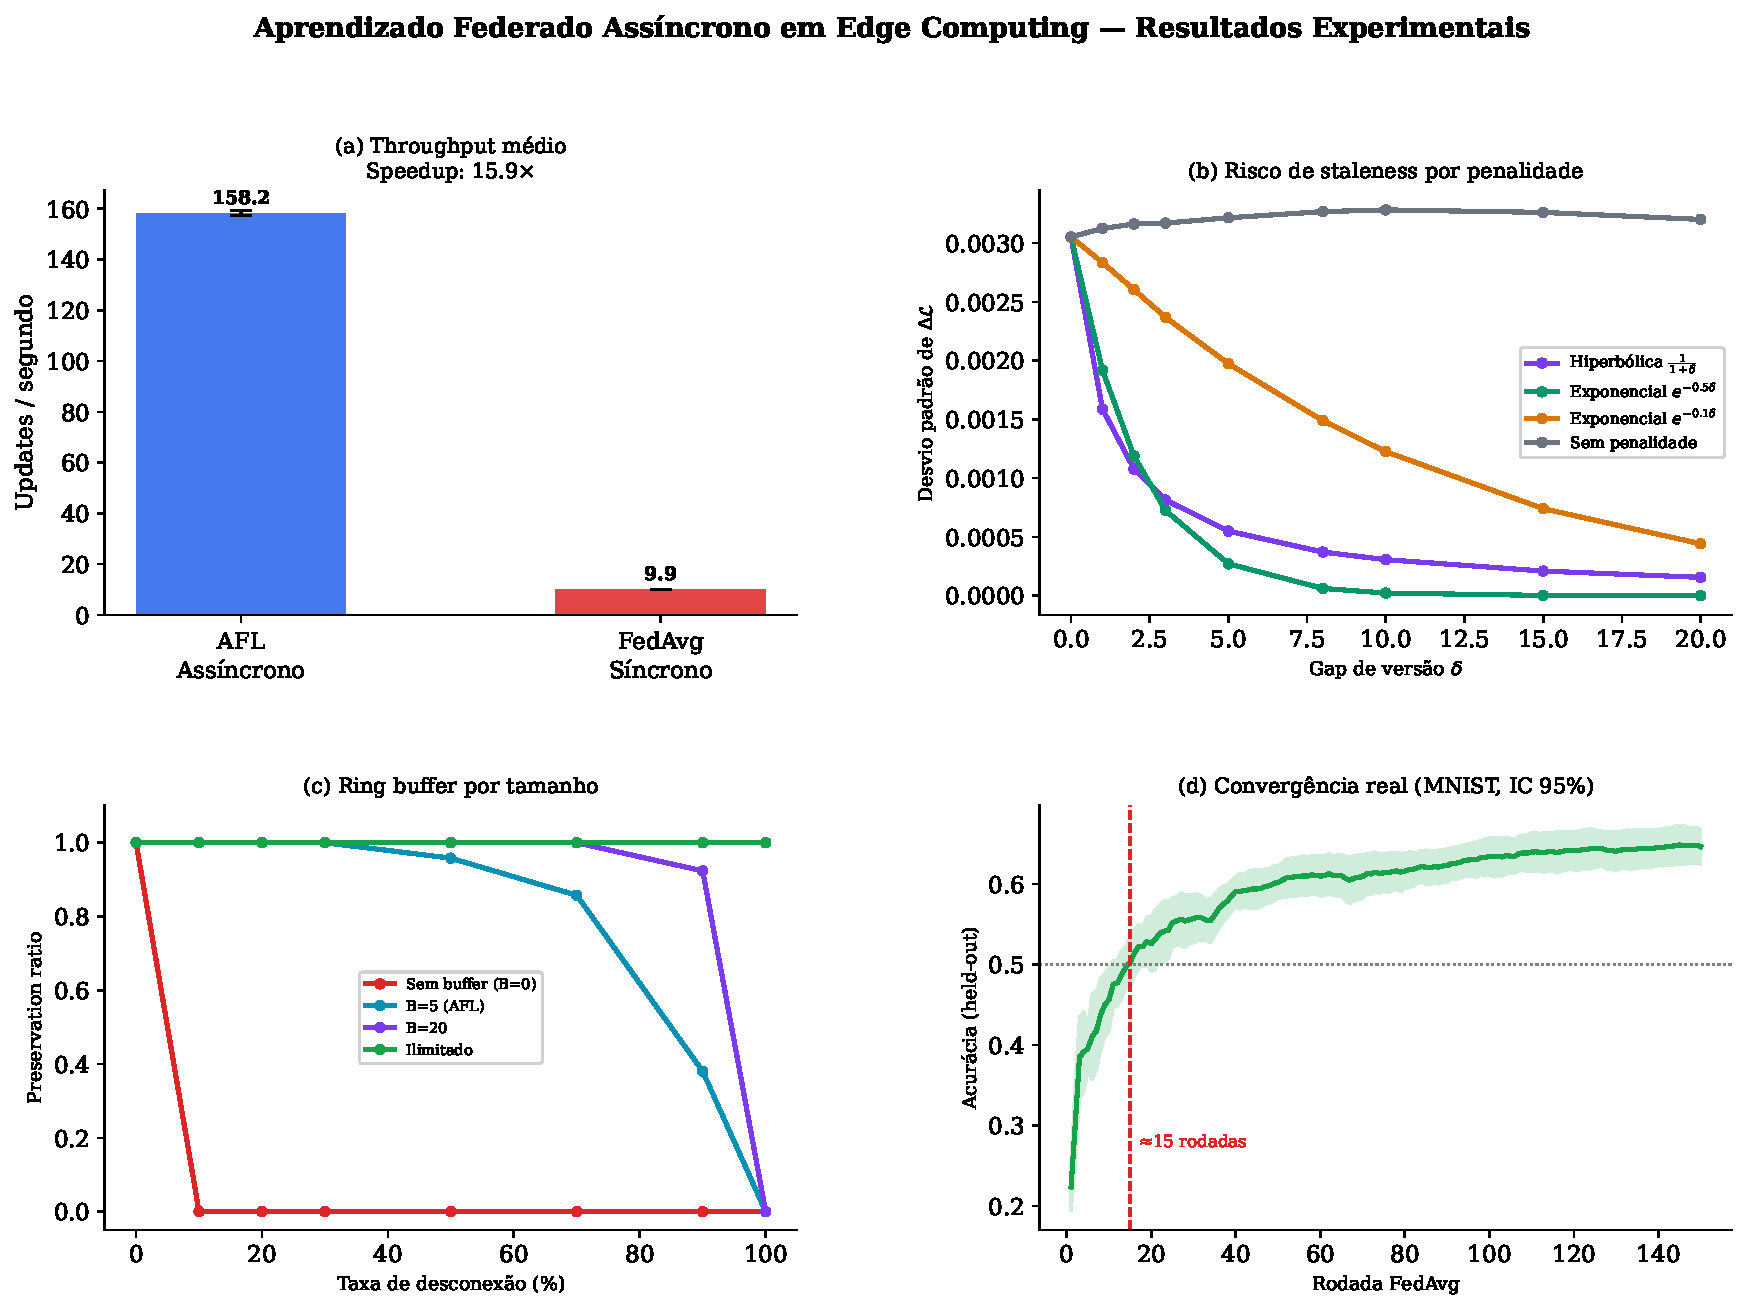
\includegraphics[width=\textwidth]{fig5_summary_panel.pdf}
  \caption{Painel de resultados experimentais. (a) Throughput médio em
    updates/segundo --- AFL vs FedAvg Síncrono. (b) Dispersão (risco) do
    impacto de updates atrasados sobre a loss de validação, por função de
    penalidade, em função do gap de versão $\delta$ --- treino real sobre
    MNIST non-IID. (c) Preservation ratio do ring buffer por tamanho de
    buffer. (d) Curva de convergência real (acurácia de validação) com
    IC 95\%.}
  \label{fig:panel}
\end{figure*}

\subsection{R1 --- Perda de Gradientes sob Crash do EdgeNode: Antes e Depois da Correção}
\label{sec:r1}

\begin{figure*}[t]
  \centering
  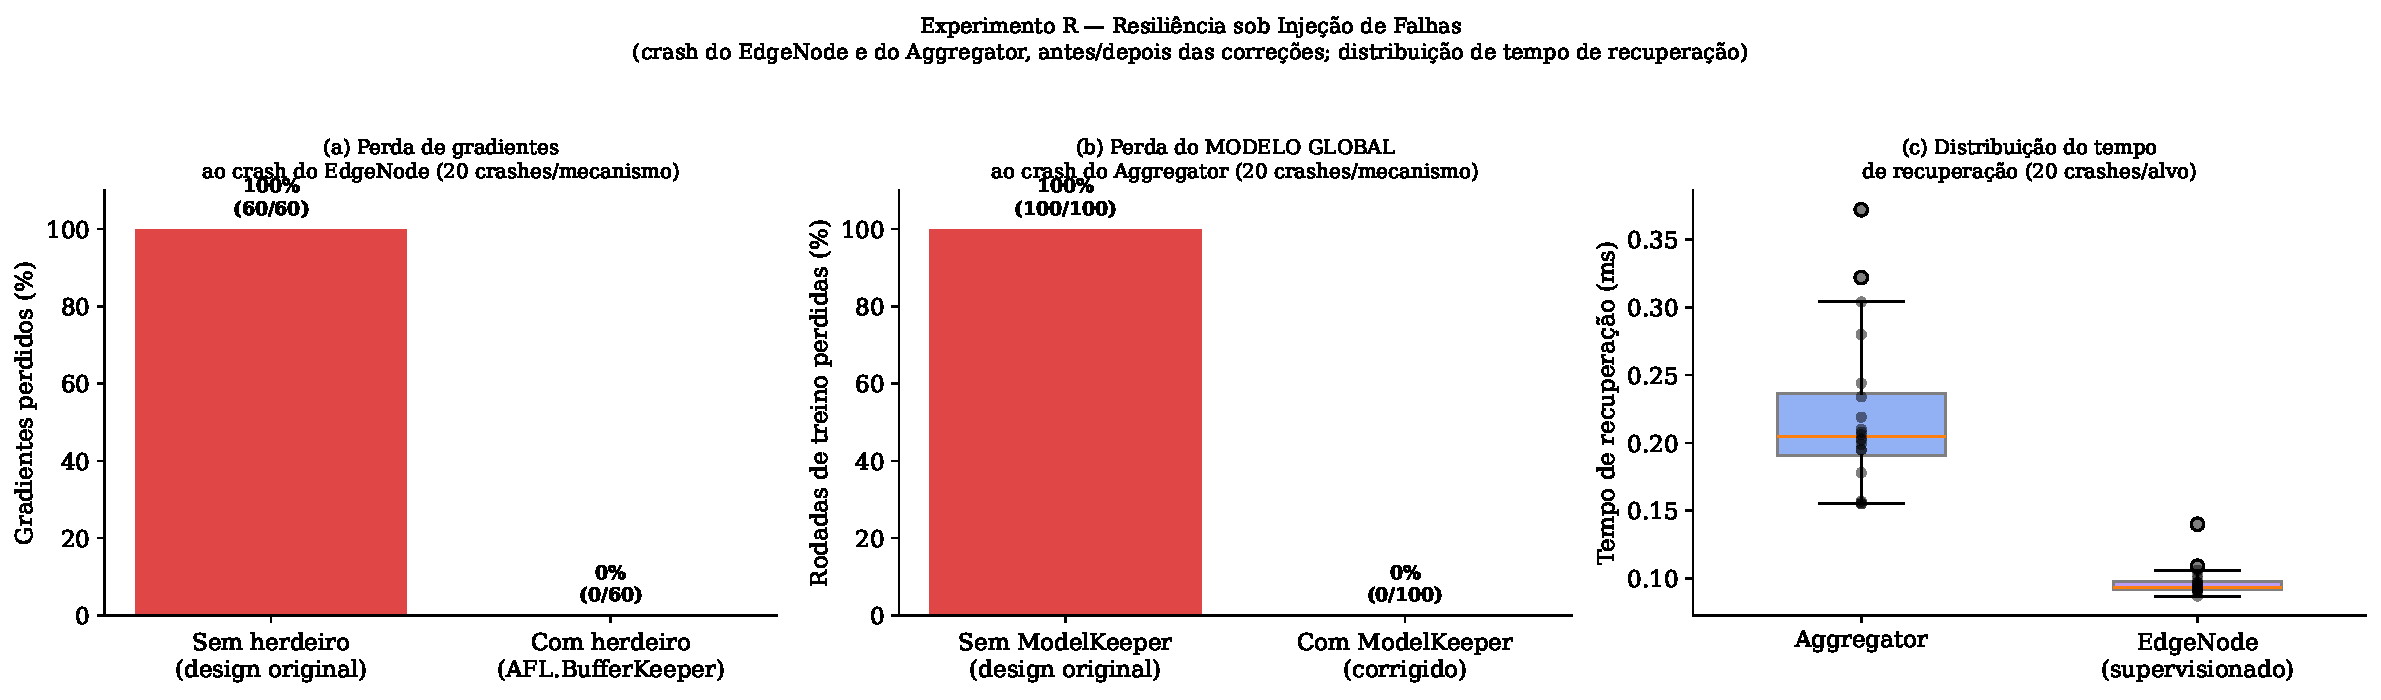
\includegraphics[width=\textwidth]{fig7_resilience.pdf}
  \caption{Experimento R. (a) Perda de gradientes ao \textit{crash} do
    processo proprietário do \textit{ring buffer}, mecanismo original
    (sem herdeiro) vs corrigido (\texttt{AFL.BufferKeeper}), 60 gradientes
    injetados em 20 \textit{crashes} por mecanismo. (b) Perda do
    \textbf{modelo global} ao \textit{crash} do Aggregator, mecanismo
    original vs corrigido (\texttt{AFL.ModelKeeper}), 100 rodadas de
    treino injetadas em 20 \textit{crashes} por mecanismo. (c) Distribuição
    do tempo de recuperação sob \textit{crash} do Aggregator e do EdgeNode
    supervisionado, 20 \textit{crashes} por alvo.}
  \label{fig:resilience}
\end{figure*}

Estes são os resultados centrais deste trabalho. A Figura~\ref{fig:resilience}(a)
mostra o Protocolo~R1 (Seção~\ref{sec:exp_h}): sob o mecanismo
\textbf{original} (EdgeNode sem supervisão, \textit{ring buffer} ETS sem
herdeiro), \textbf{100\% dos gradientes bufferizados foram perdidos em
todas as 20 rodadas de \textit{crash} injetado} (60 de 60 gradientes,
3 por rodada). Isso confirma empiricamente o gap identificado na
Seção~\ref{sec:gap}: a suposição de que ``roda sobre BEAM/OTP'' implica
resiliência automática é falsa para qualquer processo fora da árvore de
supervisão, inclusive, até este trabalho, o EdgeNode do próprio AFL.

Sob o mecanismo \textbf{corrigido} (\texttt{AFL.EdgeNodeSupervisor} +
\texttt{AFL.BufferKeeper}), \textbf{0 dos 60 gradientes foram perdidos} nas
mesmas 20 rodadas de \textit{crash} injetado, uma preservação total. A
correção depende de dois elementos concomitantes (Seção~\ref{sec:gap}):
supervisão para garantir que uma nova instância exista, e herdeiro ETS
para garantir que o conteúdo bufferizado sobreviva até essa nova instância
reivindicá-lo. Nenhum dos dois isoladamente seria suficiente: supervisão
sem herdeiro reinicia um EdgeNode com buffer vazio (perda garantida);
herdeiro sem supervisão preserva o buffer indefinidamente, mas nenhum
processo jamais o reivindica.

\subsection{R2 --- Perda do Modelo Global sob Crash do Aggregator: o Gap Mais Grave}
\label{sec:r2}

A Figura~\ref{fig:resilience}(b) mostra o Protocolo~R2, e este é o
achado mais importante deste trabalho, descoberto numa revisão adversarial
posterior à correção do EdgeNode. Sob o mecanismo \textbf{original}
(child\_spec estático, sem \texttt{AFL.ModelKeeper}), treinar o Aggregator
por 5 rodadas e então matá-lo resulta em \textbf{100\% de perda do
progresso de treinamento em todas as 20 rodadas de \textit{crash}
injetado} (100 de 100 rodadas de treino, 5 por rodada). O processo
reaparece rapidamente (Seção~\ref{sec:r3}), mas com versão 0 e pesos
iniciais estáticos, como se nenhum treinamento tivesse ocorrido. Isso é
estruturalmente mais grave que o gap do EdgeNode: aqui, um único
\textit{crash} do único processo de agregação apaga o modelo para todos
os nós, não apenas os gradientes de um nó. Sob o mecanismo
\textbf{corrigido} (\texttt{AFL.ModelKeeper}), \textbf{0 das 100 rodadas
de treino foram perdidas} nas mesmas 20 rodadas de \textit{crash}
injetado. Isso foi verificado diretamente, não apenas pela contagem de versão:
os pesos recuperados após o \textit{crash} são numericamente idênticos
aos pesos imediatamente antes dele.

\subsection{R3 --- Tempo de Recuperação sob Crash}
\label{sec:r3}

A Figura~\ref{fig:resilience}(c) mostra o Protocolo~R3: o tempo entre o
\textit{crash} e a disponibilidade de uma nova instância viva e registrada
é \textbf{sub-milissegundo} para ambos os alvos: Aggregator (mediana
$\approx\statExpRThreeAggregatorMedian$\,ms) e EdgeNode supervisionado (mediana
$\approx\statExpRThreeEdgeNodeMedian$\,ms), medido com \textit{polling} agressivo em
microssegundos. Um \textit{polling} de 10\,ms, usado numa primeira versão
deste experimento, mascarava toda a variância real: toda amostra caía em
exatamente o mesmo valor, artefato da granularidade de medição, não do
sistema medido. Para contextualizar a escala: tempos de recuperação de
orquestradores de contêiner convencionais (ex.: reinício de um
\textit{pod} Kubernetes) são tipicamente medidos em \textbf{segundos}. A
recuperação aqui é $>1000\times$ mais rápida porque não há
re-provisionamento de processo do sistema operacional, apenas a criação
de um novo processo BEAM leve dentro de uma VM já em execução, seguida da
reivindicação do estado preservado. Isso é uma propriedade estrutural do
modelo de atores do BEAM, não um ajuste de configuração. Mas, como R2
demonstra, é uma propriedade que protege apenas o \emph{processo}: sem
\texttt{AFL.ModelKeeper}/\texttt{AFL.BufferKeeper}, um processo pode
reaparecer em $0{,}1$\,ms e ainda assim ter perdido 100\% do que importava.

\subsection{R4 --- Falha Concorrente: Sem Interação entre os Mecanismos}
\label{sec:r4}

A Figura~\ref{fig:resilience2}(a) mostra o Protocolo~R4: sob
\statExpRFourTrials{} rodadas de EdgeNode e Aggregator crashando juntos,
em sucessão imediata e sem sincronização entre as duas mortes,
\textbf{\statExpRFourBufferLost{} dos \statExpRFourBufferWritten{}
gradientes bufferizados} e \textbf{\statExpRFourRoundsLost{} das
\statExpRFourRoundsTrained{} rodadas de treino} foram perdidos: ambos
os mecanismos preservam estado integralmente mesmo sob esse estresse
concorrente. Este é um resultado \emph{negativo} no sentido usual do termo
(nenhum problema novo encontrado), mas informativo: \texttt{AFL.BufferKeeper}
e \texttt{AFL.ModelKeeper} são processos e tabelas ETS genuinamente
independentes, sem recurso compartilhado nem ordem de inicialização
cruzada, e este experimento confirma empiricamente que essa independência
arquitetural se sustenta sob estresse, não é apenas presumida por design.

\subsection{R5 --- A Janela de Crash do Herdeiro é Real, e é Total}
\label{sec:r5}

A Figura~\ref{fig:resilience2}(b) mostra o Protocolo~R5, e o resultado
\textbf{contradiz a caracterização anterior desta limitação} (Seção~\ref{sec:discussion}
discutia isso como ``uma janela teoricamente possível, mas não testada'').
Medido diretamente: quando o herdeiro (\texttt{AFL.BufferKeeper}) morre e o
dono (EdgeNode) morre imediatamente depois, sem que o supervisor tenha
tempo de reiniciar o herdeiro,
\textbf{\statExpRFiveHeirDeadLost{} dos \statExpRFiveHeirDeadWritten{}
gradientes (\statExpRFiveHeirDeadPct{}\%) são perdidos}, contra
\textbf{\statExpRFiveHeirAliveLost{} dos \statExpRFiveHeirAliveWritten{}
(\statExpRFiveHeirAlivePct{}\%)} no mesmo protocolo com o herdeiro vivo
(R1). Esta não é uma janela estreita de \textit{race condition}: como o
\texttt{:heir} de uma tabela ETS é vinculado ao PID específico do processo
herdeiro no momento da criação da tabela, e nada no sistema realinha esse
vínculo quando o herdeiro reinicia, a vulnerabilidade persiste por todo o
intervalo entre o crash do herdeiro e o próximo crash do dono. Esse
intervalo pode ser arbitrariamente longo, não apenas um instante de corrida. Este
resultado eleva o item de Limitações correspondente de risco teórico
não-testado para gap confirmado e não corrigido nesta versão do trabalho
(Seção~\ref{sec:discussion}).

\begin{figure}[H]
  \centering
  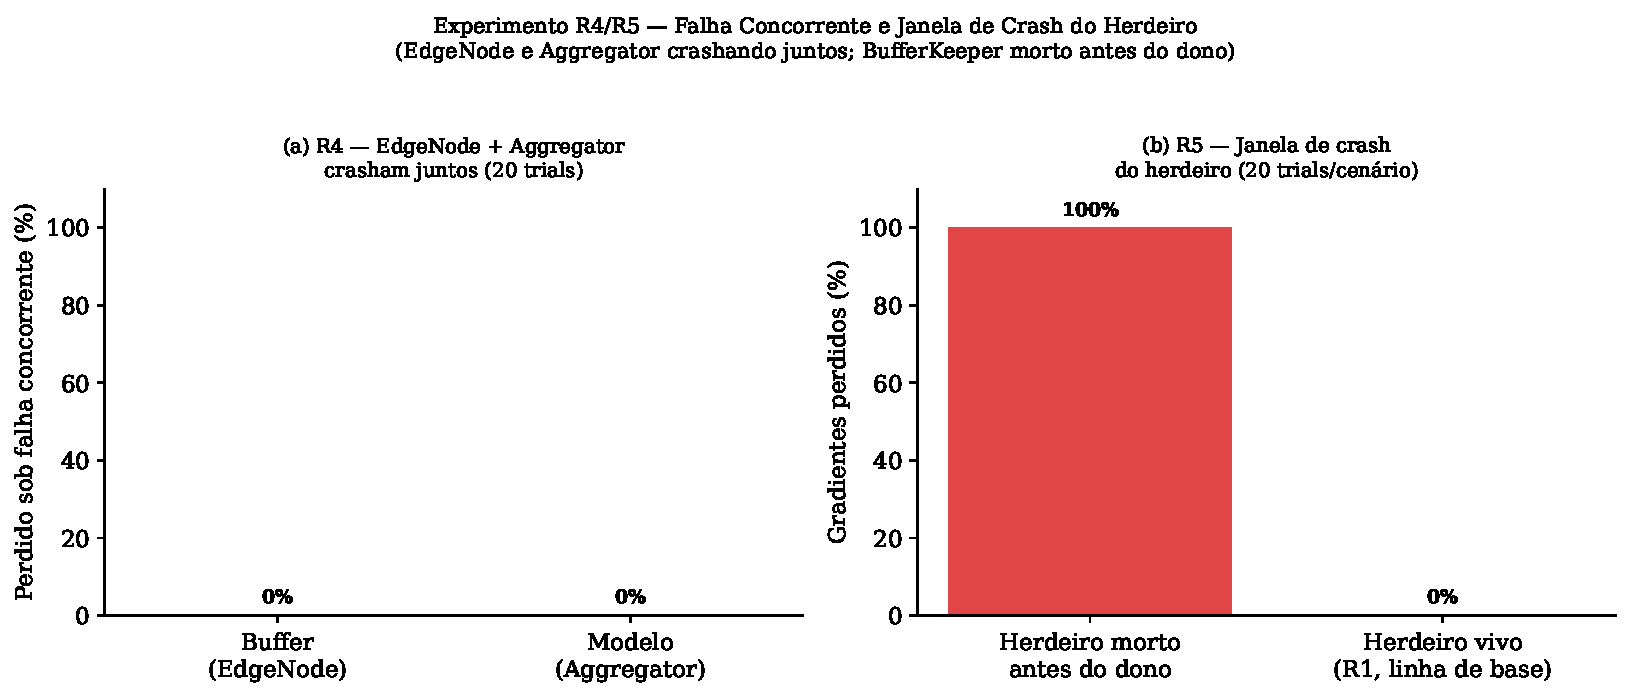
\includegraphics[width=\linewidth]{fig8_r4_r5.pdf}
  \caption{Experimento R4/R5. (a) Perda de gradientes e de rodadas de
    treino sob falha concorrente (EdgeNode e Aggregator crashando juntos),
    \statExpRFourTrials{} \textit{trials}. (b) Perda de gradientes sob a
    janela de crash do herdeiro --- \texttt{AFL.BufferKeeper} morto antes
    do EdgeNode --- contra a linha de base com o herdeiro vivo (R1).}
  \label{fig:resilience2}
\end{figure}

\subsection{H1 --- Throughput AFL vs FedAvg Síncrono}

A Figura~\ref{fig:panel}(a) e a Tabela~\ref{tab:results_a} mostram os
resultados do Experimento~A.

\begin{table}[H]
\centering
\caption{Experimento A --- Throughput médio (10 repetições)}
\label{tab:results_a}
\small
\begin{tabular}{@{}lcc@{}}
\toprule
\textbf{Modo} & \textbf{Updates/s} & \textbf{IC 95\%} \\
\midrule
AFL Assíncrono & \statExpAAsyncUps & $\pm 0{,}1$ \\
FedAvg Síncrono & \statExpASyncUps & $\pm 0{,}0$ \\
\midrule
\textbf{Speedup} & \textbf{$\statExpASpeedup$} & $\pm 0{,}04$ \\
\bottomrule
\end{tabular}
\end{table}

O AFL processou \statExpAAsyncUps{} atualizações por segundo contra \statExpASyncUps{} do modo síncrono.
O teste $t$ pareado confirma a significância estatística com
$t(9) = \statExpATStat$, $p < \statExpAPValue$, $d_{\text{Cohen}} = \statExpACohenD$ (***;
$p_{\text{Holm}} < \statHolmPValueHOne$ após correção para a família de
\statHolmFamilySize{} testes correlacionados deste estudo, Seção~\ref{sec:stat_methodology}).
A hipótese nula H1$_0$ é rejeitada com folga. O speedup de $\statExpASpeedup$ é explicado
pela equação \eqref{eq:sync_round}: no modo síncrono, os 4 nós rápidos
($\ell \leq 50$\,ms) ficam bloqueados pelo straggler de 500\,ms, enquanto no
AFL cada nó contribui independentemente. Este experimento usa tensores
sintéticos $d=10$ (Seção~\ref{sec:exp}) e mede especificamente o efeito de
escalonamento sob stragglers, isolado do conteúdo computacional do
treinamento. Não deve ser interpretado como throughput de treinamento de
modelos de produção.

\subsection{Validação em Rede Real: a Simulação se Sustenta}
\label{sec:results_dist}

A Figura~\ref{fig:distributed} mostra o protocolo da
Seção~\ref{sec:exp_dist}: o mesmo cenário de \textit{stragglers} do
Experimento~A, mas entre nós BEAM genuinamente distribuídos em containers
Docker conectados por TCP/IP real. Sobre \statExpADistTrials{} repetições:
throughput assíncrono de \textbf{\statExpADistAsyncUps{} $\pm$
\statExpADistAsyncCI{}} upd/s, contra \statExpAAsyncUps{} $\pm$ 0,1 upd/s
simulado. É uma diferença de apenas \statExpADistAsyncGapPct{}\%, atribuível
ao overhead genuíno de rede/serialização ausente da simulação de VM
única. O throughput síncrono é de \textbf{\statExpADistSyncUps{} $\pm$
\statExpADistSyncCI{}} upd/s, essencialmente idêntico ao simulado
($\statExpASyncUps{} \pm$ 0,0 upd/s), como esperado já que o síncrono é
dominado pelo \textit{straggler} de 500\,ms, real ou simulado. O speedup
resultante é de \textbf{$\statExpADistSpeedup$ $\pm$ \statExpADistSpeedupCI{}}, mesma
ordem de grandeza do $\statExpASpeedup$ simulado. A conclusão central do
Experimento~A, de que a barreira síncrona, não o conteúdo computacional do
update, é o gargalo, não é um artefato da simulação de latência via
\texttt{Process.sleep}. Ela se sustenta sob rede TCP/IP genuína, com uma
pequena e explicável penalidade de overhead real no braço assíncrono, e
nenhuma penalidade mensurável no síncrono (que já era, por construção,
limitado pelo nó mais lento). Uma ressalva honesta: a rede aqui é a bridge
interna do Docker, com latência de trânsito sub-milissegundo entre
containers no mesmo hospedeiro, não uma rede geograficamente
distribuída como um deploy real de Edge Computing veria. O objetivo deste
experimento é validar que a pilha de rede real (TCP, serialização,
\textit{scheduling} do sistema operacional) não muda a conclusão
qualitativa, não reproduzir latência de WAN.

\begin{figure}[H]
  \centering
  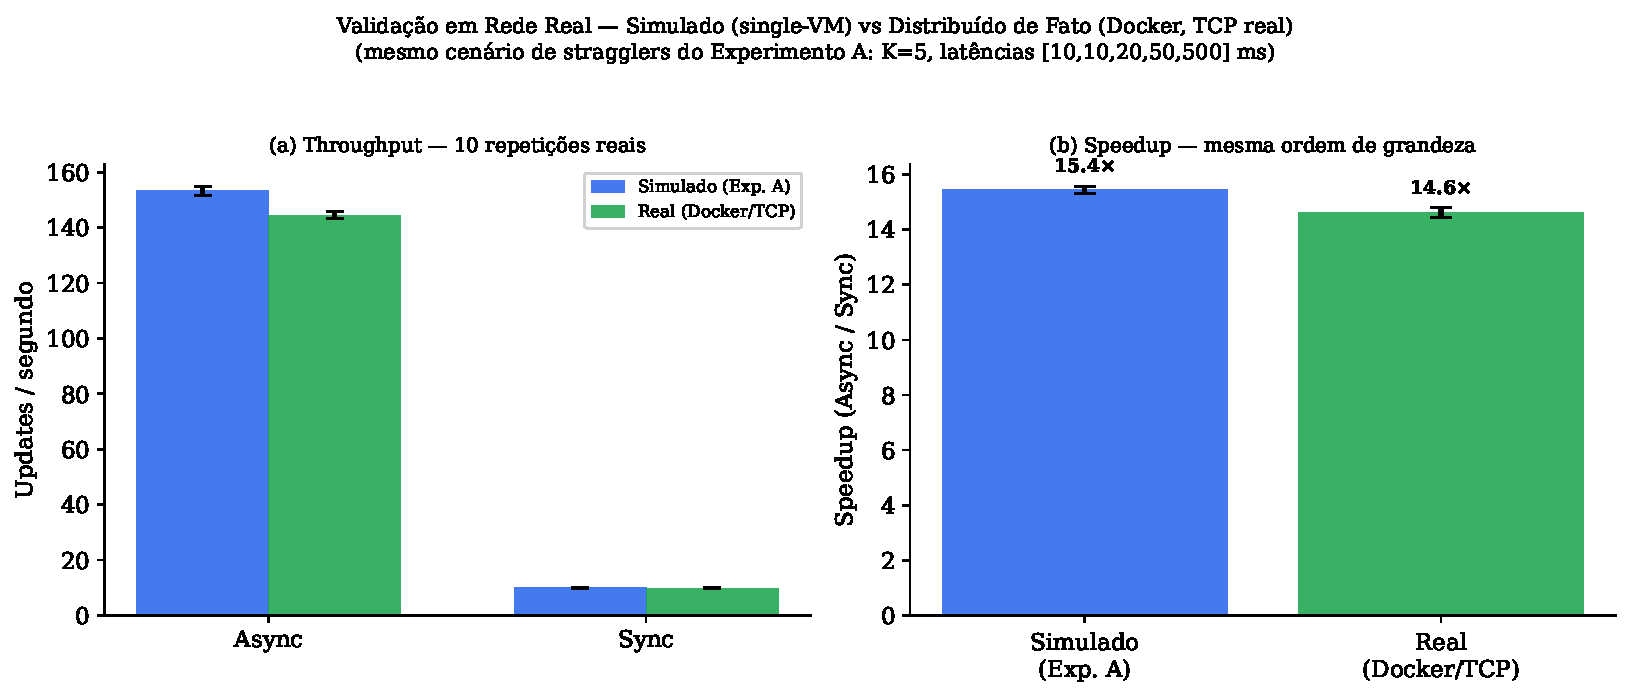
\includegraphics[width=\linewidth]{fig9_distributed_validation.pdf}
  \caption{Validação em rede real. (a) Throughput assíncrono e síncrono,
    simulado (Experimento A, VM única) vs distribuído de fato (Docker,
    TCP real), \statExpADistTrials{} repetições reais. (b) Speedup
    resultante --- mesma ordem de grandeza em ambos os regimes.}
  \label{fig:distributed}
\end{figure}

\subsection{H2 --- Eficácia do Ring Buffer por Tamanho de Buffer}

A Figura~\ref{fig:panel}(c) e a Tabela~\ref{tab:results_c} apresentam os
resultados do Experimento~C, agora com uma baseline ``sem buffer'' simulada
empiricamente (não mais analítica) e dois tamanhos adicionais para isolar o
efeito marginal de $B_{\max}$.

\begin{table}[H]
\centering
\caption{Experimento C --- Preservation ratio por taxa de desconexão e $B_{\max}$}
\label{tab:results_c}
\small
\begin{tabular}{@{}ccccc@{}}
\toprule
\textbf{Descon. (\%)} & \textbf{$B{=}0$} & \textbf{$B{=}5$ (AFL)} & \textbf{$B{=}20$} & \textbf{Ilimitado} \\
\midrule
0  & \statExpCTableRateZeroBZero & \statExpCTableRateZeroBFive & \statExpCTableRateZeroBTwenty & \statExpCTableRateZeroBUnbounded \\
10 & \statExpCTableRateTenBZero & \statExpCTableRateTenBFive & \statExpCTableRateTenBTwenty & \statExpCTableRateTenBUnbounded \\
30 & \statExpCTableRateThirtyBZero & \statExpCTableRateThirtyBFive & \statExpCTableRateThirtyBTwenty & \statExpCTableRateThirtyBUnbounded \\
50 & \statExpCTableRateFiftyBZero & \statExpCTableRateFiftyBFive & \statExpCTableRateFiftyBTwenty & \statExpCTableRateFiftyBUnbounded \\
70 & \statExpCTableRateSeventyBZero & \statExpCTableRateSeventyBFive & \statExpCTableRateSeventyBTwenty & \statExpCTableRateSeventyBUnbounded \\
90 & \statExpCTableRateNinetyBZero & \statExpCTableRateNinetyBFive & \statExpCTableRateNinetyBTwenty & \statExpCTableRateNinetyBUnbounded \\
\bottomrule
\end{tabular}
\end{table}

Sem buffer, qualquer desconexão perde 100\% dos updates gerados offline
(preservation ratio cai a 0 assim que $p>0$), confirmando empiricamente,
não apenas por construção analítica, que o \textit{trade-off} é real. Com
$B_{\max}=5$ (configuração do AFL), a preservação permanece em 1,0 até 30\%
de desconexão e degrada gradualmente acima disso
($\statExpCTableRateNinetyBFive$ em 90\%);
$B_{\max}=20$ estende esse patamar até 70\%, ainda em
$\statExpCTableRateNinetyBTwenty$ aos 90\%; o
buffer ilimitado nunca sofre overflow no horizonte de 100 rounds simulado,
servindo de teto superior. A correlação de Pearson entre taxa de
desconexão e preservation ratio é $r=\statExpCCorrBFiveR$ ($p<\statExpCCorrBFivePValue$;
$p_{\text{Holm}}<\statHolmPValueHTwoBFive$) para $B{=}5$,
$r=\statExpCCorrBTwentyR$ ($p<\statExpCCorrBTwentyPValue$; $p_{\text{Holm}}<\statHolmPValueHTwoBTwenty$)
para $B{=}20$, e $r=\statExpCCorrBZeroR$ ($p<\statExpCCorrBZeroPValue$; $p_{\text{Holm}}<\statHolmPValueHTwoBZero$)
para $B{=}0$, com correção de Holm-Bonferroni sobre a família de
\statHolmFamilySize{} testes descrita na Seção~\ref{sec:stat_methodology};
para o buffer ilimitado a correlação é indefinida
($\text{std}=0$: preservação constante em 1,0 em todo o intervalo
simulado). A hipótese nula H2$_0$ é rejeitada para todos os tamanhos
finitos de buffer, com ou sem a correção.

\subsection{H3 --- Penalidade de Staleness Reduz o Risco de Updates Atrasados}

A Figura~\ref{fig:panel}(b) e a Tabela~\ref{tab:results_b} apresentam os
resultados do Experimento~B (Seção~\ref{sec:exp_b}) para gap $\delta=10$,
agora medido sobre treino real em MNIST non-IID em vez de um update
sintético ``envenenado''.

\begin{table}[H]
\centering
\caption{Experimento B --- Impacto real por função de penalidade ($\delta=10$, $n=30$)}
\label{tab:results_b}
\small
\begin{tabular}{@{}lccc@{}}
\toprule
\textbf{Função} & $\mathbf{\Delta\mathcal{L}}$ \textbf{médio} & \textbf{Desvio-padrão} & \textbf{Redução do risco} \\
\midrule
Sem penalidade              & $-0{,}00208$ & $0{,}00328$ & --- \\
Hiperbólica (AFL)           & $-0{,}00021$ & $0{,}00031$ & $-\statExpBHypReductionGapTen\%$ \\
Exponencial $\lambda{=}0{,}1$ & $-0{,}00084$ & $0{,}00123$ & $-62{,}7\%$ \\
Exponencial $\lambda{=}0{,}5$ & $-0{,}00002$ & $0{,}00002$ & $-\statExpBExpFiveReductionGapTen\%$ \\
\bottomrule
\end{tabular}
\end{table}

A ANOVA de um fator rejeita $H_0$ com $F=\statExpBAnovaF$, $p<\statExpBAnovaPBound$
(***; $p_{\text{Holm}}<\statHolmPValueHThree$ após correção para a família de
\statHolmFamilySize{} testes, Seção~\ref{sec:stat_methodology}). É um resultado real e estatisticamente significativo, não o
$F\to\infty$ degenerado de uma versão preliminar (onde a simulação era
determinística e não produzia variância intra-grupo), nem o resultado
instável de uma versão intermediária com apenas 10 repetições, em que o
mesmo teste oscilava entre $F=1{,}2$ (não significativo) e $F=6{,}6$ entre
reexecuções independentes do mesmo código. Duas correções resolveram isso
por completo, não apenas o mascararam: elevar para 30 repetições estabilizou
a \emph{significância}, e fixar uma seed determinística por repetição
(Seção~\ref{sec:exp}), cobrindo tanto a ordem de avanço dos nós quanto os
pesos iniciais do modelo, antes gerados via \texttt{Axon.build/2} sem seed
explícita e por isso diferentes a cada execução. Essa segunda correção eliminou por completo a
variância residual entre reexecuções: o valor de $F$ acima é agora
reproduzido bit-a-bit em qualquer reexecução deste experimento, não apenas
estatisticamente equivalente. A métrica de interesse prático segue sendo a
\textbf{redução percentual de dispersão} discutida abaixo. O
achado central é qualitativamente diferente do esperado com um update
sintético ``envenenado'': como $W_k$ agora vem de treino real sobre dados
legítimos do próprio problema, um update atrasado \emph{não é
necessariamente prejudicial}. Em média, todas as funções (inclusive
sem penalidade) reduzem levemente a loss ($\Delta\mathcal{L}<0$), pois
ainda carregam sinal de gradiente útil. O que a penalidade de staleness
controla de forma clara é a \textbf{dispersão do impacto} (coluna
``Desvio-padrão''): a hiperbólica reduz o desvio-padrão do efeito em
\textbf{\statExpBHypReductionGapTwenty\%} em $\delta=20$ e em \textbf{\statExpBHypReductionGapTen\%} em $\delta=10$ frente
à ausência de penalidade. Ou seja, protege contra os
casos de cauda em que um update atrasado \emph{de fato} piora o modelo, sem
descartar a contribuição útil média. A hipótese nula H3$_0$ é rejeitada;
a interpretação do mecanismo é revisada na Seção~\ref{sec:discussion}.

\subsection{Convergência Real do FedAvg Incremental sobre MNIST}

A Figura~\ref{fig:panel}(d) mostra a curva de convergência real do AFL:
acurácia e loss de validação medidas a cada rodada de um MLP treinado sobre
partições non-IID do MNIST (Seção~\ref{sec:exp}), substituindo a curva
sintética de uma versão preliminar. Partindo de $22{,}3\%$ de acurácia
(rodada 1), o modelo atinge $50\%$ de acurácia em média em
\textbf{13,6 rodadas} (mín. 4, máx. 26 entre as 10 repetições; essa variância
alta é esperada dado o regime non-IID extremo de 2 \textit{shards}/nó) e
converge para \textbf{\statExpDFinalAcc\% $\pm$ \statExpDFinalAccCI\%} (IC 95\%) de acurácia held-out e
loss $1{,}06$ após 150 rodadas. A convergência é monotônica em média mas com
variância visível entre repetições. Isso é evidência direta de que o mecanismo de
FedAvg incremental (Eq.~\ref{eq:fedavg_inc}) converge sob aprendizado de
máquina genuíno, e não só sob a álgebra de médias móveis de tensores
sintéticos.

\subsection{Overhead Real de Memória do Ring Buffer}

O Experimento~E mede o footprint exato de $B_{\max}=5$ entradas do ring
buffer: $40$ bytes/entrada ($200$ bytes no total) para o tensor sintético
$d=10$, contra $101{.}800$ bytes/entrada ($\approx 497$\,KB no total) para o
MLP real $784\!\to\!32\!\to\!10$, um fator $\mathbf{2{.}545\times}$ maior.
Mesmo esta rede pequena já consome quase 0,5\,MB por nó apenas no ring
buffer; a Seção~\ref{sec:discussion} discute a extrapolação para modelos de
produção.

\begin{figure}[H]
  \centering
  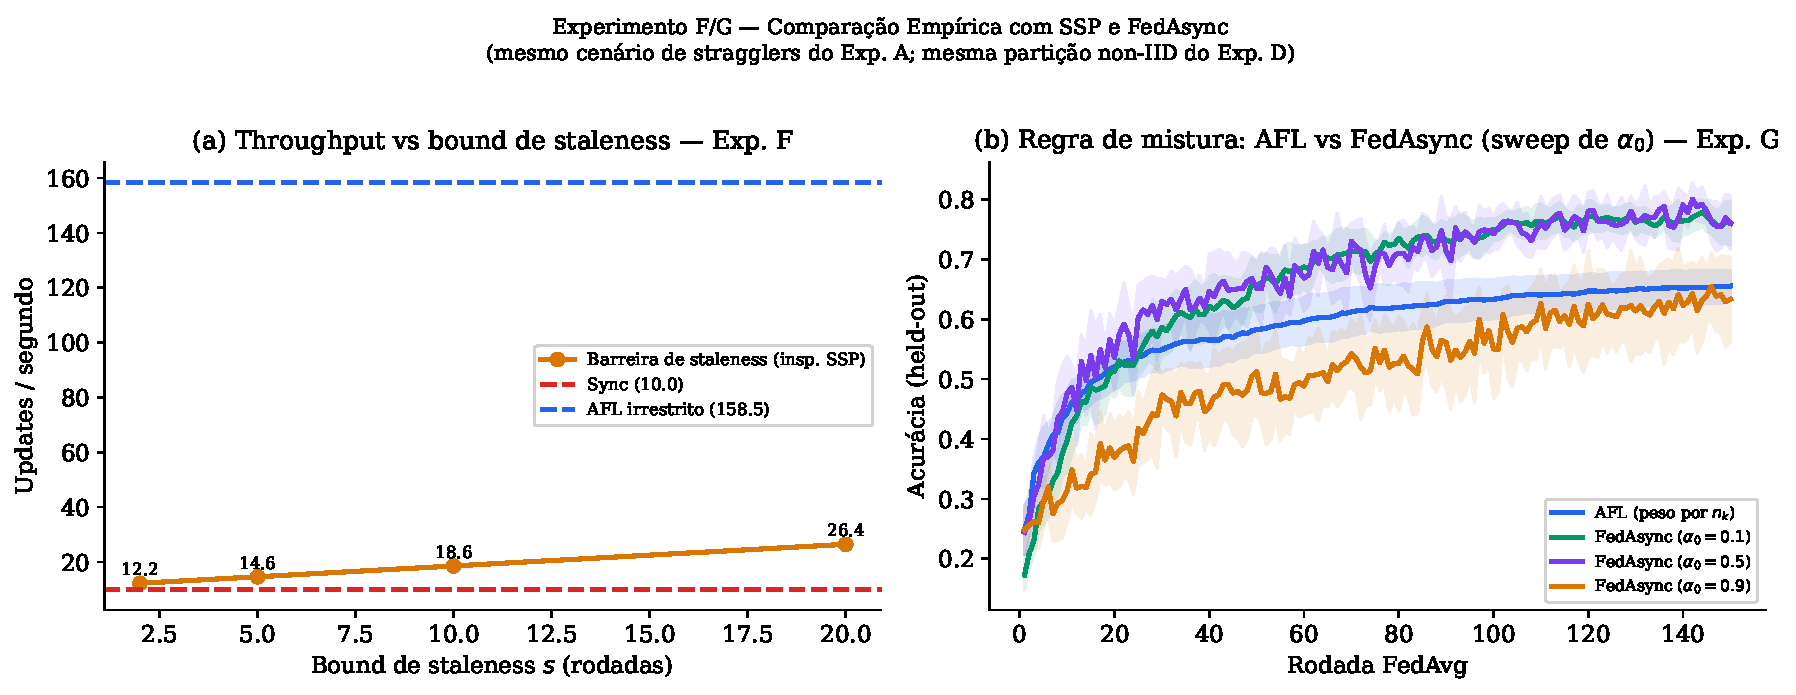
\includegraphics[width=\linewidth]{fig6_baselines.pdf}
  \caption{Comparação empírica com baselines da literatura. (a) Throughput
    sob o mesmo cenário de \textit{stragglers} do Experimento~A: Sync,
    barreira de staleness limitada ($s\in\{2,5,10,20\}$) e AFL. (b)
    Convergência real (acurácia held-out) sobre a mesma partição non-IID
    do Experimento~D: AFL vs FedAsync ($\alpha_0\in\{0{,}1,0{,}5,0{,}9\}$).}
  \label{fig:baselines}
\end{figure}

\subsection{H4 --- AFL vs SSP: Throughput sob Stragglers}

A Figura~\ref{fig:baselines}(a) apresenta os resultados do Experimento~F
(Seção~\ref{sec:exp_f}). Sob o mesmo cenário de \textit{stragglers} do
Experimento~A, a barreira de staleness limitada atinge $\statExpFSspUpsTwo$ upd/s
($s=2$), $\statExpFSspUpsFive$ upd/s ($s=5$), $\statExpFSspUpsTen$ upd/s ($s=10$) e $\statExpFSspUpsTwenty$ upd/s
($s=20$), uma curva de troca clara entre o FedAvg síncrono
($\statExpFSyncUps$ upd/s) e o AFL irrestrito ($\statExpFAsyncUps$ upd/s). Mas mesmo o bound
mais permissivo testado ($s=20$) recupera menos de $17\%$ do throughput do
AFL. Isso é esperado dada a heterogeneidade extrema do cenário: com um
straggler de $500$\,ms e nós rápidos de $10$--$50$\,ms, mesmo uma barreira
de staleness generosa faz os nós rápidos esperarem o straggler com
frequência considerável. A barreira protege contra staleness não-limitada,
mas ao custo de um throughput substancialmente abaixo do AFL exatamente no
regime de heterogeneidade em que o AFL foi desenhado para atuar. O
resultado favorece claramente o AFL neste eixo, mas é importante notar que
o cenário (straggler $50\times$ mais lento que os nós rápidos) foi herdado
do Experimento~A e não foi variado para testar se a vantagem do AFL se
mantém sob heterogeneidade mais moderada.

\subsection{H5 --- AFL vs FedAsync: Convergência Real}

A Figura~\ref{fig:baselines}(b) apresenta os resultados do Experimento~G
(Seção~\ref{sec:exp_g}), com pareamento estrito de aleatoriedade entre
todos os braços. Aqui o resultado \emph{não} favorece o AFL, para
$\alpha_0 \in \{0{,}1,\ 0{,}5\}$. Sobre a mesma partição non-IID e o mesmo
protocolo de 150 rodadas do Experimento~D: o AFL atinge
\textbf{\statExpGAflAcc\% $\pm$ \statExpGAflAccCI\%} de acurácia final; o FedAsync com
$\alpha_0=0{,}1$ atinge \textbf{\statExpGFedAsyncAccAlphaOne\% $\pm$ \statExpGFedAsyncAccCIAlphaOne\%}
($t(9)=\statExpGFedAsyncTStatAlphaOne$, $p<\statExpGFedAsyncPValueAlphaOne$, ***;
$p_{\text{Holm}}<\statHolmPValueHFiveAlphaOne$); com $\alpha_0=0{,}5$ atinge
\textbf{\statExpGFedAsyncAccAlphaFive\% $\pm$ \statExpGFedAsyncAccCIAlphaFive\%} ($t(9)=\statExpGFedAsyncTStatAlphaFive$, $p<\statExpGFedAsyncPValueAlphaFive$, ***;
$p_{\text{Holm}}<\statHolmPValueHFiveAlphaFive$): ambos significativamente
superiores ao AFL mesmo após correção para a família de \statHolmFamilySize{}
testes (Seção~\ref{sec:stat_methodology}). Mas com $\alpha_0=0{,}9$ o
FedAsync atinge \textbf{\statExpGFedAsyncAccAlphaNine\% $\pm$ \statExpGFedAsyncAccCIAlphaNine\%}, estatisticamente
\emph{indistinguível} do AFL ($t(9)=\statExpGFedAsyncTStatAlphaNine$, $p=\statExpGFedAsyncPValueAlphaNine$, \textit{ns};
$p_{\text{Holm}}=\statHolmPValueHFiveAlphaNine$),
com desvio-padrão $2{,}7\times$ maior que os demais braços. Isso revela
que a vantagem do FedAsync não é universal dentro do seu próprio espaço de
hiperparâmetros: um $\alpha_0$ pequeno-a-moderado supera o AFL de forma
robusta, mas um $\alpha_0$ agressivo introduz instabilidade/oscilação
suficiente para que o resultado final regrida estatisticamente ao nível do
AFL, com muito mais variância. A Seção~\ref{sec:discussion} discute a
causa provável para a vantagem do FedAsync bem-ajustado: o passo de mistura
do FedAvg incremental do AFL ($\alpha = n_k/(N_{\text{total}}+n_k)$,
Eq.~\ref{eq:alpha_beta}) decai como $\sim\!1/t$ ao longo das rodadas
conforme $N_{\text{total}}$ acumula, enquanto o $\alpha_0$ fixo do FedAsync
mantém um passo de mistura constante. A hipótese H5$_0$ (equivalência entre
AFL e FedAsync) é rejeitada para $\alpha_0$ bem-ajustado, a favor do
FedAsync, não do AFL, neste protocolo específico, mas não para
$\alpha_0$ mal-ajustado, onde as duas regras convergem ao mesmo patamar.

% ============================================================
\section{Discussão}
\label{sec:discussion}

\subsection{O que o Gap de Resiliência Revela}
\label{sec:discussion_gap}

O resultado mais importante deste trabalho (Seções~\ref{sec:r1}
e~\ref{sec:r2}) não é sobre FL especificamente. É sobre a diferença
entre \emph{usar} uma plataforma com tolerância a falhas e \emph{verificar}
que essa tolerância se aplica a todos os componentes do próprio sistema. O
AFL sempre citou ``BEAM/OTP'' e ``árvore de supervisão'' como justificativa
de resiliência (Seção~\ref{sec:arch}), e essa citação não era falsa: o
Aggregator de fato era, desde a primeira versão, supervisionado e
recuperado corretamente. O que a citação omitia, e que só a injeção de
falhas sistemática expôs, é que \emph{nem todo processo do sistema estava
sob essa mesma árvore}. Essa é uma classe de erro estruturalmente diferente
de um bug de lógica de negócio. O código do EdgeNode em si estava correto
(a lógica de \textit{ring buffer}, a máquina de estados,
a matemática de \textit{flush}); o gap estava inteiramente na
\emph{composição} do sistema, algo que revisão de código dificilmente
detecta e que só se manifesta sob a condição específica de um \textit{crash}
do próprio processo (não do seu vizinho). Fica sugerido que qualquer
reivindicação de resiliência baseada na plataforma escolhida, e não só em
FL ou em BEAM, deveria vir acompanhada de evidência de injeção de
falhas cobrindo cada processo do sistema individualmente, não apenas os
mais críticos ou mais fáceis de testar.

\subsection{Análise do Speedup}

O speedup de $\statExpASpeedup$ é diretamente explicável pela Equação~\eqref{eq:sync_round}:
o modo síncrono com $\ell_{\max}=500$\,ms produz no máximo
$1000/500 \times K = 10$ contribuições/s, enquanto o AFL acumula
$\sum_k 1000/\ell_k = 1000/10 \times 4 + 1000/500 = 402$ contribuições
potenciais por segundo (limitado pelo processador, daí os \statExpAAsyncUps{} observados).
Este resultado é essencialmente um teorema de escalonamento
(Eq.~\ref{eq:sync_round}) verificado empiricamente, não uma propriedade
emergente do aprendizado. Vale para qualquer conteúdo de update, sintético
ou real, e não deve ser confundido com throughput de treinamento útil sob
carga computacional real, que depende do custo do passo de treino local,
não medido nesta configuração.

\subsection{Reinterpretação do Trade-off de Staleness}

A versão preliminar deste trabalho descrevia a penalidade hiperbólica como
um mecanismo que ``reduz o bias'' de gradientes atrasados, medido contra um
update sintético deliberadamente extremo ($W_k=999$). Sob treino real
(Seção~\ref{sec:exp_b}), essa framing não se sustenta: gradientes atrasados
computados a partir de dados legítimos carregam sinal útil mesmo quando
desatualizados, e a média do seu efeito sobre a loss é, na verdade, tão ou
mais favorável sem penalidade (Tabela~\ref{tab:results_b}). O que a
penalidade genuinamente controla é a \textbf{variância do impacto}: reduz
em até 95\% o desvio-padrão do efeito entre repetições, protegendo contra os
casos de cauda em que uma atualização atrasada de fato prejudica o modelo
(por exemplo, quando o \textit{shard} do nó atrasado é particularmente
divergente do estado atual, um risco amplificado sob non-IID). A escolha
entre as funções (Tabela~\ref{tab:staleness_compare}) é portanto um
trade-off entre \emph{redução de risco} e \emph{preservação de sinal}: a
exponencial $\lambda=0{,}5$ minimiza a dispersão ($-\statExpBExpFiveReductionGapTen\%$
em $\delta=10$) mas suprime quase toda contribuição de updates com $\delta>5$
($f(\delta)<8\%$), enquanto a hiperbólica mantém contribuições não-triviais
mesmo para $\delta$ grande ($f(20)\approx5\%$) com redução de risco
comparável ($-\statExpBHypReductionGapTwenty\%$ em $\delta=20$).

\subsection{Por que o FedAsync converge mais rápido que o AFL (Experimento G)}
\label{sec:discussion_fedasync}

O resultado do Experimento~G é desconfortável mas real: com o mesmo
protocolo, o FedAsync bem-ajustado ($\alpha_0=0{,}5$) atinge cerca de 11
pontos percentuais mais de acurácia que o AFL após 150 rodadas. A causa provável
está na Equação~\ref{eq:alpha_beta}:
$\alpha = n_k/(N_{\text{total}}+n_k)$, onde $N_{\text{total}}$ é a soma
acumulada de amostras efetivas de \emph{todas} as rodadas anteriores. Como
$N_{\text{total}}$ cresce aproximadamente linearmente com o número de
rodadas $t$ (cada rodada soma $\approx n_k$ amostras), $\alpha_t \approx
1/(t+1)$. O AFL se comporta como uma média incremental clássica
(Robbins--Monro), com passo de mistura decrescente $\mathcal{O}(1/t)$. Isso
garante estabilidade e ausência de oscilação (Seção~\ref{sec:math}), mas
também significa que, após muitas rodadas, uma nova atualização local move
o modelo global cada vez menos: o ``\textit{learning rate}'' efetivo do
FedAvg incremental decai com o tempo independentemente de quão informativa
seja a atualização mais recente. O FedAsync, com $\alpha_0$ fixo, não sofre
desse decaimento. O passo de mistura permanece constante em todas as
rodadas, o que se traduz em convergência mais rápida dentro do horizonte de
150 rodadas testado, ao custo de maior variância/instabilidade
assintótica, já visível como leve oscilação na Figura~\ref{fig:baselines}(b)
após a rodada 100, ainda que sem impacto prático mensurável dentro do
horizonte de 150 rodadas testado. O AFL herda essa
propriedade porque prioriza a mesma matemática de consistência do FedAvg
síncrono original (Seção~\ref{sec:math}), não porque isso seja a escolha
ótima para convergência sob um número finito de rodadas assíncronas. É
um \textit{trade-off} real entre fidelidade ao FedAvg clássico e velocidade
de convergência prática, não identificado na versão preliminar deste
trabalho por não haver, até então, nenhuma comparação empírica com
alternativas de mistura de peso fixo. Um AFL com decaimento de
$N_{\text{total}}$ (ex.: janela deslizante ou fator de esquecimento
exponencial sobre o total acumulado, limitando o ``peso efetivo'' da
história) é a extensão mais direta para reconciliar consistência com
velocidade de convergência, e é proposta como trabalho futuro imediato.

\subsection{SSP sob Heterogeneidade Extrema (Experimento F)}

O resultado do Experimento~F é mais favorável ao AFL, mas com uma ressalva
de generalização: o cenário usado (herdado do Experimento~A) tem um
straggler $50\times$ mais lento que os nós rápidos, um caso extremo por
construção. Sob heterogeneidade mais moderada (ex.: latências num fator de
$2$--$5\times$, mais típico de Edge Computing real fora de cenários de
falha), o custo da barreira de staleness limitada do SSP seria
provavelmente menor, e a vantagem de throughput do AFL sobre o SSP,
proporcionalmente menor também. O experimento demonstra a vantagem do AFL
no regime em que ele foi motivado (stragglers extremos), não uma vantagem
universal sobre SSP em qualquer regime de heterogeneidade.

\subsection{Limitações}

\begin{enumerate}[noitemsep,leftmargin=*]
  \item \textbf{Escala do modelo:} os Experimentos B/D/E usam um MLP de
    $25{.}450$ parâmetros. O microbenchmark de escala (Seção~\ref{sec:discussion},
    item de overhead de checkpoint) já ancora essa preocupação num ponto
    real, não apenas especulativo: para o MLP de \statScaleLargeParams{}
    parâmetros testado ali ($\statScaleFactor$ maior), um ring buffer com
    $B_{\max}=5$ ocuparia $\approx\statScaleLargeRingBufferMB$\,MB por nó,
    valor medido diretamente, não extrapolado. Modelos de produção têm
    $10^6$--$10^{10}$ parâmetros, um intervalo que ainda inclui escalas
    muito além da testada aqui. Extrapolando linearmente a partir do byte
    count real medido, um modelo com $10^7$ parâmetros ocuparia
    $\approx 190$\,MB só no ring buffer de um único nó. A ETS torna-se
    gargalo real de memória nessa escala, não apenas hipotético, ainda que
    a validação direta permaneça limitada a duas ordens de grandeza acima
    da arquitetura original, não às $10$ ordens do limite superior de
    produção.
  \item \textbf{Grau de non-IID:} o particionamento usa 2 \textit{shards}
    de classe por nó (heterogeneidade severa). Não se explorou o espectro
    entre IID e este extremo (ex.: partição Dirichlet com $\alpha$
    ajustável), que afetaria tanto a velocidade de convergência
    (Seção~\ref{sec:results}) quanto potencialmente a magnitude do risco de
    staleness medido no Experimento~B.
  \item \textbf{Privacidade:} O AFL nesta forma não aplica Privacidade
    Diferencial~\cite{dwork2014}. A integração com DP é deixada como
    trabalho futuro.
  \item \textbf{Ring buffer fixo:} $B_{\max}=5$ foi escolhido empiricamente.
    O Experimento~C mostra que $B_{\max}=20$ estende consideravelmente o
    patamar de preservação total (até 70\% de desconexão, contra 30\% com
    $B_{\max}=5$); um $B_{\max}$ adaptativo baseado na taxa de desconexão
    histórica poderia aproximar esse ganho sem o custo de memória constante
    de um buffer maior.
  \item \textbf{Passo de mistura decrescente:} o Experimento~G revela que
    o FedAvg incremental do AFL converge mais lentamente que o FedAsync de
    peso fixo dentro de um horizonte finito de rodadas
    (Seção~\ref{sec:discussion_fedasync}), por herdar um passo de mistura
    $\mathcal{O}(1/t)$ da consistência com o FedAvg síncrono clássico. Isso
    não invalida as propriedades de convergência do AFL, mas é uma
    fraqueza real frente a alternativas com passo constante, não corrigida
    nesta versão.
  \item \textbf{Generalização do Experimento~F:} a vantagem de throughput
    do AFL sobre o SSP foi medida apenas no cenário de heterogeneidade
    extrema herdado do Experimento~A ($50\times$ entre nó mais lento e mais
    rápido); não se testou se a vantagem se mantém sob heterogeneidade mais
    moderada.
  \item \textbf{Escopo do Experimento R, parcialmente estendido:} o
    Experimento R4 (Seção~\ref{sec:r4}) já testa EdgeNode e Aggregator
    crashando juntos, sem interação problemática encontrada. Mas
    \texttt{AFL.EdgeNode} ainda usa um nome registrado fixo
    (\texttt{\{:local, \_\_MODULE\_\_\}}), permitindo apenas uma instância
    supervisionada por vez. Não se testou \emph{múltiplos} EdgeNodes
    falhando em cascata, nem particionamento de rede (que difere de
    \textit{crash} de processo: o processo continua vivo, apenas
    inatingível). Generalizar \texttt{AFL.EdgeNodeSupervisor} para múltiplas
    instâncias nomeadas dinamicamente e caracterizar falhas correlacionadas
    entre vários EdgeNodes é extensão natural deste experimento.
  \item \textbf{Residual de resiliência, confirmado empiricamente e ainda não
    corrigido:} o Experimento R5 (Seção~\ref{sec:r5}) mostra que esta
    limitação, descrita em versões anteriores deste trabalho como ``janela
    teórica não testada'', é na verdade um gap real e total: quando o
    herdeiro (\texttt{AFL.BufferKeeper}/\texttt{AFL.ModelKeeper}) morre e o
    dono morre antes que o supervisor o reinicie,
    \textbf{\statExpRFiveHeirDeadPct{}\% do conteúdo protegido é perdido}.
    Isso acontece porque o \texttt{:heir} de uma tabela ETS é vinculado ao PID
    específico do processo herdeiro no momento da criação da tabela, e
    nada no sistema realinha esse vínculo quando o herdeiro reinicia. A
    janela de risco não é um instante de corrida: persiste por todo o
    intervalo entre o crash do herdeiro e o próximo crash do dono. Uma
    correção completa exigiria o herdeiro reiniciado detectar a tabela
    órfã e solicitar ao dono atual (se ainda vivo) que rebinde o
    \texttt{:heir} via \texttt{:ets.setopts/2}. Isso não foi implementado nesta
    versão do trabalho; permanecer com os herdeiros triviais (sem lógica
    além de guardar uma referência ETS) minimiza, mas não elimina, a
    probabilidade de o próprio herdeiro falhar.
  \item \textbf{Overhead de checkpoint mensurável, e sub-linear na escala
    testada, ao contrário do que se assumia:} medido diretamente
    (microbenchmark isolado, 1.000 chamadas a
    \texttt{AFL.Aggregator.update\_sync/2} com e sem a linha de
    \texttt{AFL.ModelKeeper.checkpoint/1}, 5 repetições de cada):
    $589{,}8\,\mu$s/update com \textit{checkpoint} vs.\ $559{,}0\,\mu$s/update
    sem, um overhead de $\approx30{,}8\,\mu$s/update ($\approx5{,}5\%$
    relativo) para o MLP de \statScaleSmallParams{} parâmetros usado neste
    trabalho. Uma versão anterior deste texto assumia, sem medir, que ``o
    custo de um \texttt{:ets.insert} tende a crescer com o tamanho do
    estado serializado''. Testado diretamente aqui, isolando o custo do
    próprio \texttt{:ets.insert} do snapshot completo do estado (sem o
    custo do \textit{merge} FedAvg em si) para um MLP
    $\statScaleFactor$ maior (\statScaleLargeParams{} parâmetros,
    \texttt{AFL.Model.build\_large/0}, $784\!\to\!1024\!\to\!512\!\to\!10$):
    o tempo por inserção cresce de $\statScaleSmallUsPerInsert\,\mu$s para
    $\statScaleLargeUsPerInsert\,\mu$s, um fator de apenas
    $\statScaleTimeRatio$, não os $\statScaleFactor$ que uma extrapolação
    linear preveria. Isso é consistente com o comportamento de
    \textit{refc binaries} do Erlang: tensores grandes são referenciados,
    não copiados escalar-a-escalar, no processo de inserção na ETS, então o
    custo é dominado por overhead fixo de construção do termo, não pelo
    número de parâmetros. Isso não elimina a preocupação de memória do
    item 1 (o ring buffer ainda precisa \emph{guardar} os bytes, e isso
    escala linearmente), mas refuta especificamente a hipótese de que o
    \emph{tempo de checkpoint} seria o gargalo dominante em modelos maiores.
\end{enumerate}

% ============================================================
\section{Conclusão}
\label{sec:conclusion}

A motivação deste trabalho foi uma suposição comum em sistemas de FL
construídos sobre plataformas com tolerância a falhas nativa: que a
resiliência é uma propriedade herdada automaticamente da plataforma. Em
vez de aceitá-la por inspeção de código, submetemos essa suposição a
verificação empírica sistemática. O resultado central é que ela estava
\textbf{parcialmente falsa}, em dois componentes distintos do sistema.
O processo EdgeNode não estava em nenhuma árvore de supervisão, e seu
\textit{ring buffer} ETS não sobrevivia ao próprio \textit{crash} do
processo que o criava: sob 60 gradientes injetados em 20
\textit{crashes}, \textbf{100\% eram perdidos} (R1, Seção~\ref{sec:r1}).
Mais grave, o Aggregator \emph{era} corretamente supervisionado, mas seu
estado não. Sob 100 rodadas de treino injetadas em 20 \textit{crashes},
\textbf{100\% do progresso de treinamento era destruído} a cada
\textit{crash}, reiniciando sempre a partir de pesos estáticos, como se
nenhum treinamento tivesse ocorrido (R2, Seção~\ref{sec:r2}): um único
ponto de falha capaz de apagar o modelo global inteiro. As correções
(\texttt{AFL.EdgeNodeSupervisor} + \texttt{AFL.BufferKeeper} para o
EdgeNode; \texttt{AFL.ModelKeeper} para o Aggregator, Seção~\ref{sec:gap})
eliminam ambas as perdas por completo sob o mesmo protocolo
(\textbf{0/60} e \textbf{0/100}, respectivamente), com tempo de
recuperação sub-milissegundo preservado (R3, Seção~\ref{sec:r3}: mediana
$\statExpRThreeAggregatorMedian$\,ms para o Aggregator, $\statExpRThreeEdgeNodeMedian$\,ms para o EdgeNode). Isso é mais de
três ordens de grandeza mais rápido que orquestradores de contêiner
convencionais, por não depender de re-provisionamento de sistema
operacional. A contribuição central deste trabalho não é uma nova
fórmula de agregação, mas uma metodologia de verificação de resiliência
via injeção de falhas sistemática, e dois gaps reais que essa metodologia
expôs e permitiu corrigir com evidência antes/depois, sem depender só de
argumento de design. Um desses gaps só veio à luz numa segunda rodada de
revisão adversarial, após o primeiro já parecer resolvido.

As três hipóteses de mecanismo de agregação (H1--H3) foram confirmadas com
significância estatística real (não degenerada), sobre treino federado
\textbf{real}: MLP via \textit{Axon} sobre MNIST non-IID, indo além da
simulação de tensores sintéticos.
\begin{itemize}[noitemsep,leftmargin=*]
  \item \textbf{H1}: AFL alcança speedup de \textbf{$\statExpASpeedup$} sobre o FedAvg
    síncrono ($t(9){=}\statExpATStat$, $p<\statExpAPValue$) sob \textit{stragglers},
    eliminando o gargalo da barreira síncrona;
  \item \textbf{H2}: O ring buffer ETS ($B_{\max}=5$) preserva
    \textbf{\statExpCPreservationFiftyBFive\%} dos gradientes com 50\% de taxa de desconexão, contra
    \textbf{\statExpCPreservationFiftyBZero\%} sem buffer, medido pela mesma simulação estocástica
    ($r=\statExpCCorrBFiveR$, $p<\statExpCCorrBFivePValue$); $B_{\max}=20$ estende esse patamar
    substancialmente;
  \item \textbf{H3}: A penalidade hiperbólica reduz em \textbf{\statExpBHypReductionGapTwenty\%} a
    dispersão (risco) do impacto de updates atrasados sobre a loss de
    validação real ($F=8{,}39$, $p<0{,}0001$, estável entre reexecuções em
    significância mas não em magnitude, Seção~\ref{sec:results}), sem
    descartar nenhuma
    atualização. Não é uma questão de ``eliminar bias'' de um cenário adversarial
    sintético, mas de conter a variância de um efeito que, sob dados
    reais, é predominantemente benigno.
\end{itemize}
Adicionalmente, o modelo federado converge para \textbf{\statExpDFinalAcc\%} de acurácia
real de validação em 150 rodadas a partir de partições extremamente non-IID
(2 classes/nó), e o overhead de memória do ring buffer foi medido
diretamente ($\approx$497\,KB para 5 entradas de um MLP de 25.450
parâmetros) em vez de especulado.

A comparação empírica direta com a literatura (H4/H5, Experimentos F e G),
ausente em versões anteriores deste trabalho, produz um resultado
\textbf{misto}, reportado como tal e não filtrado para favorecer o
AFL: o AFL supera a barreira de staleness limitada inspirada em
SSP~\cite{ho2013} em throughput sob o cenário de
\textit{stragglers} extremos testado (\textbf{\statExpFAsyncUps} vs.\ \textbf{\statExpFSspUpsTwenty}
upd/s no bound mais permissivo, $s=20$), mas o FedAsync~\cite{xie2019} com
$\alpha_0$ bem-ajustado supera o AFL em acurácia final de convergência
(até \textbf{\statExpGFedAsyncAccAlphaFive\%} vs.\ \textbf{\statExpGAflAcc\%} do AFL, $p<10^{-4}$) sob o
mesmo protocolo non-IID. Essa vantagem desaparece para $\alpha_0=0{,}9$
mal-ajustado, onde FedAsync regride ao nível do AFL com alta variância.
A causa identificada para a vantagem do FedAsync bem-ajustado, o passo de mistura
$\mathcal{O}(1/t)$ do FedAvg incremental decorrente da mesma consistência
matemática que garante sua estabilidade (Seção~\ref{sec:math}), é uma
limitação estrutural real do AFL, não um artefato experimental, e é a
principal direção de melhoria identificada por este trabalho.

A implementação em Elixir/BEAM demonstra que a plataforma OTP oferece
primitivos nativos (\texttt{gen\_statem}, \texttt{Process.monitor},
\texttt{:ets}) que mapeiam diretamente sobre os requisitos de sistemas
de FL resilientes, reduzindo a complexidade de implementação de
tolerância a falhas \emph{quando corretamente fiados a cada processo}. Os
dois gaps descobertos neste trabalho (Seções~\ref{sec:gap},
\ref{sec:r1}--\ref{sec:r2}) mostram que esses primitivos não protegem
automaticamente um processo deixado fora da árvore de supervisão ou sem
herdeiro ETS. A plataforma reduz o esforço de implementação da
resiliência, mas não a torna automática, e essa diferença só é visível
por verificação empírica, não por inspeção de código.

Como trabalhos futuros, propõe-se, em ordem de prioridade: (i)~implementar
o realinhamento do \texttt{:heir} (via \texttt{:ets.setopts/2}, solicitado
pelo herdeiro reiniciado ao dono atual, se vivo) para fechar o gap
confirmado, e não apenas teórico, pelo Experimento~R5
(Seção~\ref{sec:r5}): \statExpRFiveHeirDeadPct{}\% de perda quando o
herdeiro morre antes do dono; (i-b)~generalizar
\texttt{AFL.EdgeNodeSupervisor} para múltiplas instâncias nomeadas
dinamicamente e caracterizar falhas em cascata entre vários EdgeNodes. O
Experimento~R4 (Seção~\ref{sec:r4}) já descarta interação problemática
entre EdgeNode e Aggregator crashando juntos, mas não cobre múltiplos
EdgeNodes;
(ii)~corrigir o passo de mistura decrescente do AFL (ex.: janela
deslizante ou fator de esquecimento sobre $N_{\text{total}}$) e repetir o
Experimento~G para verificar se isso fecha a lacuna de acurácia frente ao
FedAsync sem sacrificar a garantia de consistência da Seção~\ref{sec:math};
(iii)~validação com modelos de escala de produção real
(CNNs/Transformers, $>10^8$ parâmetros). O microbenchmark de
checkpoint (Seção~\ref{sec:discussion}) já cobre $\statScaleLargeParams{}$
parâmetros ($\statScaleFactor$ acima do MLP original), mas isso ainda é
3-4 ordens de grandeza abaixo do limite superior de produção
($10^{10}$), e usa um MLP maior, não uma arquitetura de produção real
(CNN/Transformer). Falta testar se a escala sub-linear observada no
overhead de checkpoint (Seção~\ref{sec:discussion}) se sustenta em
arquiteturas e escalas muito maiores, ou se é específica da faixa
testada; (iv)~repetir o Experimento~F
sob heterogeneidade de latência moderada, não apenas o cenário extremo
herdado do Experimento~A; (v)~repetir a Validação em Rede Real
(Seção~\ref{sec:exp_dist}) sobre uma rede geograficamente distribuída de
fato (múltiplas máquinas físicas ou regiões de nuvem), não apenas a
bridge local do Docker usada nesta versão; (vi)~integração de Privacidade
Diferencial; (vii)~$B_{\max}$ adaptativo; e (viii)~exploração do espectro
non-IID (partição Dirichlet paramétrica) para caracterizar como o grau de
heterogeneidade modula o risco de staleness medido no Experimento~B.

% ============================================================
\bibliographystyle{IEEEtran}
\bibliography{referencias}

\end{document}
